\documentclass[a4paper]{book}

\usepackage[hypcap=false]{caption}
\usepackage{enumitem}	% 定制enumerate标号
\usepackage{geometry}
\geometry{%
	left=2cm,%
	right=2cm,%
	top=2cm,%
	bottom=2cm,%
	bindingoffset=0cm
}
\usepackage{hyperref}
\hypersetup{
    colorlinks=true,            %链接颜色
    linkcolor=blue,             %内部链接
    filecolor=magenta,          %本地文档
    urlcolor=cyan,              %网址链接
    pdftitle={Overleaf Example},
    pdfpagemode=FullScreen,
}
\usepackage[none]{hyphenat}	% 阻止长单词分在两行
\usepackage{mathrsfs}	% 提供\mathscr字体
\usepackage[version=4]{mhchem}
\usepackage{multirow}

\RequirePackage[many]{tcolorbox}
\tcbset{
    boxed title style={colback=magenta},
	breakable,
	enhanced,
	sharp corners,
	attach boxed title to top left={yshift=-\tcboxedtitleheight,  yshifttext=-.75\baselineskip},
	boxed title style={boxsep=1pt,sharp corners},
    fonttitle=\bfseries\sffamily,
}

\definecolor{skyblue}{rgb}{0.54, 0.81, 0.94}

\newtcolorbox[auto counter, number within=chapter, number format=\arabic]{exercise}[1][]{
    title={Exercise~\thetcbcounter},
    colframe=skyblue,
    colback=skyblue!12!white,
    boxed title style={colback=skyblue},
    overlay unbroken and first={
        \node[below right,font=\small,color=skyblue,text width=.8\linewidth]
        at (title.north east) {#1};
    }
}

\newtcolorbox[auto counter, number within=chapter, number format=\arabic]{solution}[1][]{
%    top=2ex,
%    boxrule=0pt,
%    leftrule=1.4pt,
    title={Solution~\thetcbcounter},
    colframe=teal!60!green,
    colback=green!12!white,
    boxed title style={colback=teal!60!green},
    overlay unbroken and first={
        \node[below right,font=\small,color=red,text width=.8\linewidth]
        at (title.north east) {#1};
    }
}

\newcommand{\AO}{{\rm AO}}
\newcommand{\Heff}{H^{\rm eff,\pi}}
\newcommand{\Hp}{H^\prime}
\newcommand{\Sp}{S^\prime}
\newcommand{\RRR}{{\rm R}^3}
\newcommand\Figref[1]{Fig \ref{#1}}
\newcommand\Tableref[1]{Table \ref{#1}}
\newcommand{\orb}[1]{{\rm #1}}
\newcommand{\orbp}{\orb{p}}

\begin{document}

	\setcounter{chapter}{10}

	\begin{exercise}
		For the following molecules, determine the point group and the symmetry of the MOs for the $\pi$-electrons, and, using H{\"u}ckel theory, obtain the MOs and orbital energies:
		\begin{enumerate}[label=(\alph*)]
		\item {\it trans}-1,3-butadiene,
		\item ethylene,
		\item cyclobutadiene,
		\item cyclopentadienyl radical $\ce{C5H5}$,
		\item naphthalene,
		\item phenanthrene.
		\end{enumerate}
	\end{exercise}

	\begin{solution}

		\begin{enumerate}[label=(\alph*)]
	
		\item Firstly, it is easy to find that {\it trans}-1,3-butadiene belongs to the point group $\mathscr{C}_{\rm 2h}$, whose character table is listed below.
		\begin{center}
		\setlength{\abovecaptionskip}{-0.1em}
		\captionof{table}{The character table for the $\mathscr{C}_{\rm 2h}$ point group.}
		\begin{tabular}{ccccc}\hline
	$\mathscr{C}_{\rm 2h}$ & $E$ & $C_2$ & $i$ & $\sigma_h$ \\ \hline
			$A_g$	&	1	&	1	&	1	&	1	\\
			$B_g$	&	1	&	-1	&	1	&	-1	\\
			$A_u$	&	1	&	1	&	-1	&	-1	\\
			$B_u$ 	&	1	&	-1	&	-1	&	1	\\ \hline
		\end{tabular}
		\setlength{\belowcaptionskip}{-0.2em}
		\end{center}
		
		Secondly, we mark all carbon atoms as follows.
		\begin{center}
		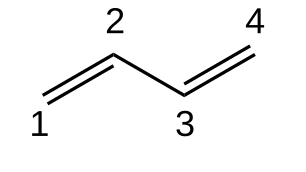
\includegraphics[scale=1.0]{./structures/exercise_1/trans-1,3-butadiene/0.png}
		\setlength{\abovecaptionskip}{-0.3em}
		\captionof{figure}{The order of carbon atoms in {\it trans}-1,3-butadiene.}
		\setlength{\belowcaptionskip}{-0.8em}
		\end{center}				

		For $\pi$-electron atomic orbitals' representation $\Gamma^{\rm AO}$, its following characters is listed below.
		\begin{center}
		\setlength{\abovecaptionskip}{-0.3em}
		\captionof{table}{The character of the $\pi$-electron atomic orbitals' representation $\Gamma^{\rm AO}$.}
		\begin{tabular}{ccccc}\hline
	$\mathscr{C}_{\rm 2h}$ & $E$ & $C_2$ & $i$ & $\sigma_h$ \\ \hline
	$\chi^{\AO}(C_i)$	&	4	&	0	&	0	&	-4	\\ \hline
		\end{tabular}\vspace*{-0.5em}
		\end{center}
		
		Relevant reduction coefficients are
		\begin{align*}
		a_g &= \frac{1}{4} \sum_{R} \chi^{\AO}(R) \chi^{A_g}(R) = \frac{1}{4} \left[ 1 \times 4 \times 1 + 1 \times 0 \times 1 + 1 \times 0 \times 1 + 1 \times (-4) \times 1 \right] = 0, \\
		b_g &= \frac{1}{4} \sum_{R} \chi^{\AO}(R) \chi^{B_g}(R) = \frac{1}{4} \left[ 1 \times 4 \times 1 + 1 \times 0 \times (-1) + 1 \times 0 \times 1 + 1 \times (-4) \times (-1) \right] = 2, \\
		a_u &= \frac{1}{4} \sum_{R} \chi^{\AO}(R) \chi^{A_u}(R) = \frac{1}{4} \left[ 1 \times 4 \times 1 + 1 \times 0 \times 1 + 1 \times 0 \times (-1) + 1 \times (-4) \times (-1) \right] = 2, \\
		b_u &= \frac{1}{4} \sum_{R} \chi^{\AO}(R) \chi^{B_u}(R) = \frac{1}{4} \left[ 1 \times 4 \times 1 + 1 \times 0 \times (-1) + 1 \times 0 \times (-1) + 1 \times (-4) \times 1 \right] = 0.
		\end{align*}
		
		Thus, we arrive at
		\begin{equation*}
			\Gamma^{\AO} = 2 \Gamma^{B_g} \oplus 2 \Gamma^{A_u}.
		\end{equation*}
		We conclude that there are two basis functions in the irreducible representation $\Gamma^{B_g}$ and $\Gamma^{A_u}$, respectively. Thus, to describe the effect of $O_R$, two suitable $2 \orbp_z$ atomic orbitals $\phi_i$ is enough.
		
		Thirdly, we inspect the transformation of $\phi_i$ under $O_R$ for the {\it trans}-1,3-butadiene, whose information is recorded below. We only list two $\phi_1$ and $\phi_2$, which is enough in current case.
		\begin{center}
		\setlength{\abovecaptionskip}{0em}
		\captionof{table}{Transformation of $\phi_i$ under $O_R$ for the {\it trans}-1,3-butadiene.}
		\begin{tabular}{ccccc}\hline
	$\mathscr{C}_{\rm 2h}$ & $O_E$ & $O_{C_2}$ & $O_i$ & $O_{\sigma_h}$ \\ \hline
			$\phi_1$	&	$\phi_1$	&	$\phi_4$	&	$-\phi_4$	&	$-\phi_1$	\\
			$\phi_2$	&	$\phi_2$	&	$\phi_3$	&	$-\phi_3$	&	$-\phi_2$	\\	\hline
		\end{tabular}
		\setlength{\belowcaptionskip}{0.5em}
		\end{center}
		
		For the irreducible representation $\Gamma^{B_g}$,
		\begin{align*}
		P^{B_g}\phi_1 &= \sum_{R} \chi^{B_g}(R) O_R \phi_1 = (O_E - O_{C_2} + O_{i} - O_{\sigma_h})\phi_1 = 2(\phi_1-\phi_4) , \\
		P^{B_g}\phi_2 &= \sum_{R} \chi^{B_g}(R) O_R \phi_2 = (O_E - O_{C_2} + O_{i} - O_{\sigma_h})\phi_2 = 2(\phi_2-\phi_3) .
		\end{align*}
		It is easy to find that they are mutually orthogonal. They can be normalized to
		\begin{align*}
		\phi^\prime_1 &= \frac{1}{\sqrt{2}} (\phi_1-\phi_4) , \\
		\phi^\prime_2 &= \frac{1}{\sqrt{2}} (\phi_2-\phi_3) .
		\end{align*}
		
		Then, the effective Hamitonian matrix elements for $\pi$ electrons can be calculated,
		\begin{align*}
		\Hp_{11} &= \int_{\RRR} \frac{1}{\sqrt{2}}(\phi_1-\phi_4) \Heff \frac{1}{\sqrt{2}}(\phi_1-\phi_4) = \frac{1}{2} (\alpha + 0 + 0 + \alpha) = \alpha, \\
		\Hp_{12} &= \int_{\RRR} \frac{1}{\sqrt{2}}(\phi_1-\phi_4) \Heff \frac{1}{\sqrt{2}}(\phi_2-\phi_3) = \frac{1}{2} (\beta - 0 - 0 + \beta) = \beta, \\
		\Hp_{22} &= \int_{\RRR} \frac{1}{\sqrt{2}}(\phi_2-\phi_3) \Heff \frac{1}{\sqrt{2}}(\phi_2-\phi_3) = \frac{1}{2} (\alpha - \beta - \beta + \alpha) = \alpha - \beta,
		\end{align*}
		viz.
		\begin{equation*}
			\Hp_{B_g} = \begin{pmatrix}
				\alpha	&	\beta \\ \beta & \alpha - \beta 
			\end{pmatrix}.
		\end{equation*}
		Next,
		\begin{align*}
			\det(\Hp_{B_g}-\varepsilon^\pi \Sp_{B_g}) = \begin{vmatrix}	
			\alpha-\varepsilon^\pi	&	\beta \\ 
			\beta & \alpha - \beta -\varepsilon^\pi	
\end{vmatrix} = \beta^2
\begin{vmatrix}
			x & 1 \\ 1 & x -1			
			\end{vmatrix} = \beta^2 ( x^x - x - 1 ) = 0,
		\end{align*}
		where
		\begin{equation*}
			x = \frac{\alpha-\varepsilon^\pi}{\beta}.
		\end{equation*}
		Current discriminant is
		\begin{equation*}
			\Delta_{B_g} = (-1)^2 - 4 \times 1 \times (-1) = 5,
		\end{equation*}				
		and then two roots are
		\begin{equation*}
			x_1 = \frac{1+\sqrt{5}}{2}, \quad x_2 = \frac{1-\sqrt{5}}{2},
		\end{equation*}
		which equal to	
		\begin{align}
			\varepsilon_1 &= \alpha - x_1 \beta = \alpha - \frac{1+\sqrt{5}}{2} \beta \approx \alpha - 1.618 \beta , \\
			\varepsilon_2 &= \alpha - x_2 \beta = \alpha - \frac{1-\sqrt{5}}{2} \beta = \alpha + \frac{\sqrt{5}-1}{2} \beta \approx \alpha + 0.618 \beta .
		\end{align}
		
		For $\Hp_{B_g}-\varepsilon^\pi_1 \Sp_{B_g}$, its reduced row echelon form is
		\begin{equation*}
			\begin{pmatrix}
				1	& \frac{-1+\sqrt{5}}{2}	\\	0	&	0
			\end{pmatrix},
		\end{equation*}
		which means
		\begin{equation*}
			\Phi_1 = -\frac{\sqrt{5}-1}{2}\phi^\prime_1 + \phi^\prime_2.
		\end{equation*}
		The sum of squares of coefficients is
		\begin{equation*}
			\sum_{i} c^2_i = (-\frac{\sqrt{5}-1}{2})^2 + 1^2 = \frac{5-\sqrt{5}}{2}.
		\end{equation*}
		
		Thus, we know
		\begin{align}
			\Phi^\pi_1 &= \sqrt{ \frac{2}{5-\sqrt{5}} } \Phi_1 = -\frac{\sqrt{5}-1}{2}\phi^\prime_1 + \phi^\prime_2 = - \sqrt{\frac{\sqrt{5}-1}{2\sqrt{5}}} \phi^\prime_1 + \sqrt{\frac{\sqrt{5}+1}{2\sqrt{5}}} \phi^\prime_2	\notag \\
			&= - \frac{1}{2}\sqrt{\frac{\sqrt{5}-1}{\sqrt{5}}}\phi_1  + \frac{1}{2}\sqrt{\frac{\sqrt{5}+1}{\sqrt{5}}} \phi_2 - \frac{1}{2}\sqrt{\frac{\sqrt{5}+1}{\sqrt{5}}} \phi_3 + \frac{1}{2}\sqrt{\frac{\sqrt{5}-1}{\sqrt{5}}} \phi_4 \notag \\
			&\approx -0.3717 \phi_1 + 0.6015 \phi_2 - 0.6015 \phi_3 + 0.3717 \phi_4.
		\end{align}
		
		Similarly, the reduced row echelon form of $\Hp_{B_g}-\varepsilon^\pi_2 \Sp_{B_g}$ is
		\begin{equation*}
			\begin{pmatrix}
				1	& \frac{-1-\sqrt{5}}{2}	\\	0	&	0
			\end{pmatrix},
		\end{equation*}		
		which means
		\begin{equation*}
			\Phi_2 = \frac{\sqrt{5}+1}{2}\phi^\prime_1 + \phi^\prime_2.
		\end{equation*}
		And then,
		\begin{align}
			\Phi^\pi_2 &= \sqrt{ \frac{2}{5+\sqrt{5}} } \Phi_2 = \frac{\sqrt{5}+1}{2}\phi^\prime_1 + \phi^\prime_2 = \sqrt{\frac{\sqrt{5}+1}{2\sqrt{5}}} \phi^\prime_1 + \sqrt{\frac{\sqrt{5}-1}{2\sqrt{5}}} \phi^\prime_2	\notag \\
			&= \frac{1}{2}\sqrt{\frac{\sqrt{5}+1}{\sqrt{5}}}\phi_1  + \frac{1}{2}\sqrt{\frac{\sqrt{5}-1}{\sqrt{5}}} \phi_2 - \frac{1}{2}\sqrt{\frac{\sqrt{5}-1}{\sqrt{5}}} \phi_3 - \frac{1}{2}\sqrt{\frac{\sqrt{5}+1}{\sqrt{5}}} \phi_4 \notag \\
			&\approx 0.6015\phi_1 + 0.3717 \phi_2 - 0.3717 \phi_3 -  0.6015\phi_4.
		\end{align}
		
		In conclusion, for the irreducible representation $\Gamma^{B_g}$, relevant results are listed below.
		
		\begin{center}
		\setlength{\abovecaptionskip}{-0.5em}
		\captionof{table}{The H{\"u}ckel MOs in the irreducible representation $\Gamma^{B_g}$ of {\it trans}-1,3-butadiene.}
		\begin{tabular}{ccc}\hline
		  order	&	eigenvalue		& 	eigenfunction	\\ \hline
			1	&$\alpha-1.618\beta$& 	$-0.3717 \phi_1 + 0.6015 \phi_2 - 0.6015 \phi_3 + 0.3717 \phi_4$ \\
			2	&$\alpha+0.618\beta$& 	$0.6015\phi_1 + 0.3717 \phi_2 - 0.3717 \phi_3 -  0.6015\phi_4$\\ \hline
		\end{tabular}
		\end{center}
		
		In the same way, for the irreducible representation $\Gamma^{A_u}$,
		\begin{align*}
		P^{A_u}\phi_1 &= \sum_{R} \chi^{A_u}(R) O_R \phi_1 = (O_E + O_{C_2} - O_{i} - O_{\sigma_h})\phi_1 = 2(\phi_1+\phi_4) , \\
		P^{A_u}\phi_2 &= \sum_{R} \chi^{A_u}(R) O_R \phi_2 = (O_E + O_{C_2} - O_{i} - O_{\sigma_h})\phi_2 = 2(\phi_2+\phi_3) .
		\end{align*}
		It is easy to find that they are mutually orthogonal, too. They can be normalized to
		\begin{align*}
		\phi^\prime_3 &= \frac{1}{\sqrt{2}} (\phi_1+\phi_4) , \\
		\phi^\prime_4 &= \frac{1}{\sqrt{2}} (\phi_2+\phi_3) .
		\end{align*}
		Then, the effective Hamiltonian can be constructed, viz.
		\begin{equation*}
			\Hp_{A_u} = \begin{pmatrix}
				\alpha	&	\beta \\ \beta & \alpha + \beta 
			\end{pmatrix}.
		\end{equation*}
		Next,
		\begin{align*}
			\det(\Hp_{A_u}-\varepsilon^\pi \Sp_{A_u}) = \begin{vmatrix}	
			\alpha-\varepsilon^\pi	&	\beta \\ 
			\beta & \alpha + \beta -\varepsilon^\pi	
\end{vmatrix} = \beta^2
\begin{vmatrix}
			x & 1 \\ 1 & x +1			
			\end{vmatrix} = \beta^2 ( x^x + x - 1 ) = 0.
		\end{align*}
		Current discriminant is
		\begin{equation*}
			\Delta_{A_u} = 1^2 - 4 \times 1 \times (-1) = 5,
		\end{equation*}		
		and then two roots are
		\begin{equation*}
			x_3 = \frac{-1+\sqrt{5}}{2}, \quad x_4 = \frac{-1-\sqrt{5}}{2},
		\end{equation*}
		which equal to
		\begin{align}
			\varepsilon_3 &= \alpha - x_3 \beta = \alpha - \frac{-1+\sqrt{5}}{2} \beta \approx \alpha - 0.618 \beta , \\
			\varepsilon_4 &= \alpha - x_4 \beta = \alpha - \frac{-1-\sqrt{5}}{2} \beta = \alpha + \frac{\sqrt{5}+1}{2} \beta \approx \alpha + 1.618 \beta .
		\end{align}
		
		For $\Hp_{A_u}-\varepsilon^\pi_3 \Sp_{A_u}$, its reduced row echelon form is
		\begin{equation*}
			\begin{pmatrix}
				1	& \frac{1+\sqrt{5}}{2}	\\	0	&	0
			\end{pmatrix},
		\end{equation*}		
		which means
		\begin{equation*}
			\Phi_3 = -\frac{\sqrt{5}+1}{2}\phi^\prime_3 + \phi^\prime_4.
		\end{equation*}
		Thus,
		\begin{align}
			\Phi^\pi_3 &= \sqrt{ \frac{2}{5+\sqrt{5}} } \Phi_3 = -\sqrt{\frac{\sqrt{5}+1}{2\sqrt{5}}} \phi^\prime_3 + \sqrt{\frac{\sqrt{5}-1}{2\sqrt{5}}} \phi^\prime_4 \notag	\\
			&= -\frac{1}{2}\sqrt{\frac{\sqrt{5}+1}{\sqrt{5}}}\phi_1  + \frac{1}{2}\sqrt{\frac{\sqrt{5}-1}{\sqrt{5}}} \phi_2 + \frac{1}{2}\sqrt{\frac{\sqrt{5}-1}{\sqrt{5}}} \phi_3 - \frac{1}{2}\sqrt{\frac{\sqrt{5}+1}{\sqrt{5}}} \phi_4 \notag \\
			&\approx -0.6015 \phi_1 + 0.3717 \phi_2 + 0.3717 \phi_3 - 0.6015 \phi_4.
		\end{align}
		
		For $\Hp_{A_u}-\varepsilon^\pi_4 \Sp_{A_u}$, its reduced row echelon form is
		\begin{equation*}
			\begin{pmatrix}
				1	& \frac{1-\sqrt{5}}{2}	\\	0	&	0
			\end{pmatrix},
		\end{equation*}		
		which means
		\begin{equation*}
			\Phi_4 = \frac{\sqrt{5}-1}{2}\phi^\prime_3 + \phi^\prime_4.
		\end{equation*}
		Thus,		
		\begin{align}
			\Phi^\pi_4 &= \sqrt{ \frac{2}{5-\sqrt{5}} } \Phi_4 = \sqrt{\frac{\sqrt{5}-1}{2\sqrt{5}}} \phi^\prime_3 + \sqrt{\frac{\sqrt{5}+1}{2\sqrt{5}}} \phi^\prime_4 \notag	\\
			&= \frac{1}{2}\sqrt{\frac{\sqrt{5}-1}{\sqrt{5}}}\phi_1  + \frac{1}{2}\sqrt{\frac{\sqrt{5}+1}{\sqrt{5}}} \phi_2 + \frac{1}{2}\sqrt{\frac{\sqrt{5}+1}{\sqrt{5}}} \phi_3 + \frac{1}{2}\sqrt{\frac{\sqrt{5}-1}{\sqrt{5}}} \phi_4 \notag \\
			&\approx 0.3717 \phi_1 + 0.6015 \phi_2 + 0.6015 \phi_3 + 0.3717 \phi_4.
		\end{align}
		
		In conclusion, for the irreducible representation $\Gamma^{A_u}$, relevant results are listed below.
		
		\begin{center}
		\setlength{\abovecaptionskip}{-0.5em}
		\captionof{table}{The H{\"u}ckel MOs in the irreducible representation $\Gamma^{A_u}$ of {\it trans}-1,3-butadiene.}
		\begin{tabular}{ccc}\hline
		  order	&	eigenvalue		& 	eigenfunction	\\ \hline
			1	&$\alpha-0.618\beta$& 	$-0.6015 \phi_1 + 0.3717 \phi_2 + 0.3717 \phi_3 - 0.6015 \phi_4$ \\
			2	&$\alpha+1.618\beta$& 	$0.3717\phi_1 + 0.6015 \phi_2 +0.6015 \phi_3 + 0.3717\phi_4$  \\	 \hline
		\end{tabular}
		\end{center}
		
		Now, we have obtained all results, which are shown as following.
		
		\begin{center}
		\setlength{\abovecaptionskip}{-0.5em}
		\captionof{table}{The H{\"u}ckel MOs in all irreducible representations of {\it trans}-1,3-butadiene.}
		\begin{tabular}{ccccccc}\hline
		order 	& orbital energy & irrep & $c_1$ & $c_2$ & $c_3$ &$c_4$ \\ \hline
			1	&	$\alpha+1.618\beta$	&	$A_u$	&	0.3717	&	0.6015	&	0.6015	&	0.3717	\\
			2	&	$\alpha+0.618\beta$	&	$B_g$	&	0.6015	&	0.3717	&	-0.3717	&	-0.6015	\\
			3	&	$\alpha-0.618\beta$	&	$A_u$	&	0.6015	&	-0.3717	&	-0.3717	&	0.6015	\\
			4	&	$\alpha-1.618\beta$	&	$B_g$	&	0.3717	&	-0.6015	&	0.6015	&	-0.3717	\\ \hline
		\end{tabular}
		\end{center}
		
		Besides, their phase diagrams have been painted in \Figref{fig:phase_diagram_1}. They obey the rule that the less nodal planes are, the lower orbital energy is.
		
		\begin{center}
		\begin{tabular}{cccc}
			\begin{minipage}[t]{0.22\linewidth}
			\centering
			\setlength{\abovecaptionskip}{0.5em}
			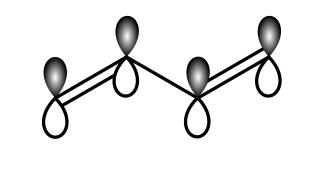
\includegraphics[scale=0.95]{./structures/exercise_1/trans-1,3-butadiene/4.png}
			\captionof*{figure}{$\varepsilon = \alpha + 1.618\beta$}
			\end{minipage} & 
			\begin{minipage}[t]{0.18\linewidth}
			\setlength{\abovecaptionskip}{0.5em}
			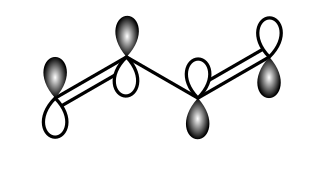
\includegraphics[scale=0.95]{./structures/exercise_1/trans-1,3-butadiene/2.png}
			\captionof*{figure}{$\varepsilon = \alpha + 0.618\beta$}
			\end{minipage} &
			\begin{minipage}[t]{0.22\linewidth}
			\centering
			\setlength{\abovecaptionskip}{0.5em}
			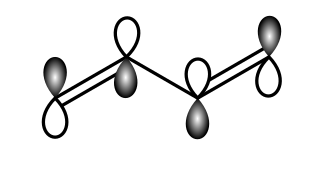
\includegraphics[scale=0.95]{./structures/exercise_1/trans-1,3-butadiene/3.png}
			\captionof*{figure}{$\varepsilon = \alpha - 0.618\beta$}
			\end{minipage} & 
			\begin{minipage}[t]{0.18\linewidth}
			\setlength{\abovecaptionskip}{0.5em}
			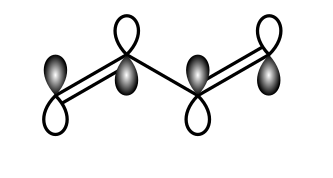
\includegraphics[scale=0.95]{./structures/exercise_1/trans-1,3-butadiene/1.png}
			\captionof*{figure}{$\varepsilon = \alpha - 1.618\beta$}
			\end{minipage}
		\end{tabular}				
		\captionof{figure}{Phase diagrams of these H{\"u}ckel MOs of {\it trans}-1,3-butadiene. Black bubbles mean plus phase while white ones mean minus phase. The color is used just for determining relative phase.}\label{fig:phase_diagram_1}
		\end{center}
		
		In the end, we conclude that for {\it trans}-1,3-butadiene, its ground state $\pi$-electron configuration is $(a_u)^2(b_g)^2$ and its delocalization energy is $2\times(1.618\beta+0.618\beta)-4\beta=0.472\beta$.
		
		\item 22222222222222222
		
		
		\begin{center}
		\begin{tabular}{ccccc}\hline
	$\mathscr{D}_{\rm 2}$ & $E$ & $C_{2z}$ & $C_{2y}$ & $C_{2x}$ \\ \hline
			$A$		&	1	&	1	&	1	&	1	\\
			$B_1$	&	1	&	1	&	-1	&	-1	\\
			$B_2$	&	1	&	-1	&	1	&	-1	\\
			$B_3$ 	&	1	&	-1	&	-1	&	1	\\ \hline
		\end{tabular}
		\end{center}
		
		
		\begin{center}
		\begin{tabular}{ccccc}\hline
	$\mathscr{D}_{\rm 2}$ & $E$ & $C_{2z}$ & $C_{2y}$ & $C_{2x}$  \\ \hline
	$\chi^{\AO}(C_i)$	&	2	&	0	&	0	&	-2	\\ \hline
		\end{tabular}
		\end{center}
		
		\begin{align*}
		a &= \frac{1}{4} \sum_{R} \chi^{\AO}(R) \chi^{A}(R) = \frac{1}{4} \left[ 1 \times 2 \times 1 + 1 \times 0 \times 1 + 1 \times 0 \times 1 + 1 \times (-2) \times 1 \right] = 0, \\
		b_1	&= \frac{1}{4} \sum_{R} \chi^{\AO}(R) \chi^{B_1}(R) = \frac{1}{4} \left[ 1 \times 2 \times 1 + 1 \times 0 \times 1 + 1 \times 0 \times (-1) + 1 \times (-2) \times (-1) \right] = 1, \\
		b_2	&= \frac{1}{4} \sum_{R} \chi^{\AO}(R) \chi^{B_2}(R) = \frac{1}{4} \left[ 1 \times 2 \times 1 + 1 \times 0 \times (-1) + 1 \times 0 \times 1 + 1 \times (-2) \times (-1) \right] = 1, \\
		b_3	&= \frac{1}{4} \sum_{R} \chi^{\AO}(R) \chi^{B_3}(R) = \frac{1}{4} \left[ 1 \times 2 \times 1 + 1 \times 0 \times (-1) + 1 \times 0 \times (-1) + 1 \times (-2) \times 1 \right] = 0.
		\end{align*}
		
		\begin{equation*}
			\Gamma^{\AO} = \Gamma^{B_1} \oplus \Gamma^{B_2}.
		\end{equation*}
		
		\begin{center}
		\begin{tabular}{ccccc}\hline
	$\mathscr{D}_{\rm 2}$ & $E$ & $C_{2z}$ & $C_{2y}$ & $C_{2x}$ \\ \hline
			$\phi_1$	&	$\phi_1$	&	$\phi_2$	&	$-\phi_2$	&	$-\phi_1$	\\	\hline
		\end{tabular}
		\end{center}
		
		\begin{equation*}
		P^{B_1}\phi_1 = \sum_{R} \chi^{B_1}(R) O_R \phi_1 = (O_E + O_{C_{2z}} - O_{C_{2y}} - O_{C_{2x}})\phi_1 = \phi_1 +\phi_2 - (-\phi_2) - (-\phi_1) = 2(\phi_1 + \phi_2) .
		\end{equation*}
		
		\begin{equation*}
		\phi^\prime_1 = \frac{1}{2}(\phi_1 + \phi_2) .
		\end{equation*}
		
		\begin{equation*}
			\Heff = ( \alpha + \beta ).
		\end{equation*}
		
		\begin{align}
			\Psi^pi_1 &= \phi^\prime_1 = \frac{1}{2}(\phi_1 + \phi_2) \\
			&\approx 0.7071 \phi_1 + 0.7071 \phi_2.
		\end{align}
		
		
		\begin{equation*}
		P^{B_2}\phi_1 = \sum_{R} \chi^{B_2}(R) O_R \phi_1 = (O_E - O_{C_{2z}} + O_{C_{2y}} - O_{C_{2x}})\phi_1 = \phi_1 - \phi_2 + (-\phi_2) + (-\phi_1) = 2(\phi_1 - \phi_2) .
		\end{equation*}
		
		\begin{equation*}
		\phi^\prime_2 = \frac{1}{2}(\phi_1 - \phi_2) .
		\end{equation*}
		
		\begin{equation*}
			\Heff = ( \alpha - \beta ).
		\end{equation*}
		
		\begin{align}
			\Psi^pi_1 &= \phi^\prime_1 = \frac{1}{2}(\phi_1 - \phi_2) \\
			&\approx 0.7071 \phi_1 - 0.7071 \phi_2.
		\end{align}
		
		Thus, we obtain all results, which are shown as following.
		
		\begin{center}
		\begin{tabular}{ccccc}\hline
		order 	& orbital energy & irrep & $c_1$ & $c_2$ \\ \hline
			1	&	$\alpha+\beta$	&	$B_1$	&	0.7071	&	-0.7071	\\
			2	&	$\alpha-\beta$	&	$B_2$	&	0.7071	&	-0.7071	\\ \hline
		\end{tabular}
		\end{center}
		
		\begin{center}
		\begin{tabular}{cccc}
			\begin{minipage}[t]{0.2\linewidth}
			\centering
			\setlength{\abovecaptionskip}{0.5em}
			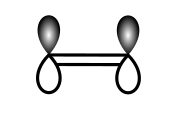
\includegraphics[scale=1]{./structures/exercise_1/ethylene/1.png}
			\captionof*{figure}{$\varepsilon = \alpha + \beta$}
			\end{minipage} & 
			\begin{minipage}[t]{0.11\linewidth}
			\setlength{\abovecaptionskip}{0.5em}
			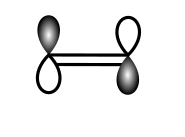
\includegraphics[scale=1]{./structures/exercise_1/ethylene/2.png}
			\captionof*{figure}{$\varepsilon = \alpha - \beta$}
			\end{minipage}
		\end{tabular}				
		\captionof{figure}{Phase diagrams of these H{\"u}ckel MOs. Black bubbles mean plus phase while white ones mean minus phase. The color is used just for determining relative phase.}\label{fig:phase_diagram_2}
		\end{center}
		
		
		
		\item This solution is designed for cyclobutadiene anion instead of just cyclobutadiene which is the prototypical antiaromatic hydrocarbon with 4 $\pi$ electrons. Its rectangular structure is the result of a pseudo-(or second order) Jahn–Teller effect, which distorts the molecule and lowers its symmetry, converting the triplet to a singlet ground state. This distortion indicates that the $\pi$ electrons are localized, in agreement with H{\"u}ckel's rule which predicts that a $\pi$-system of 4 electrons is not aromatic. This information is excerpted from \url{https://en.wikipedia.org/wiki/Cyclobutadiene}.
		
		Firstly, it is easy find that cyclobutadiene anion belongs to the point group $\mathscr{D}_{\rm 4h}$. However, it has only 4 $\pi$-electrons. Just $\mathscr{D}_{\rm 4}$ is good enough and its character table is shown in \Tableref{tab:chatab_3}.
		\begin{center}
		\setlength{\abovecaptionskip}{0em}
		\captionof{table}{The character table for the $\mathscr{D}_{\rm 4}$ point group.}\label{tab:chatab_3}
		\begin{tabular}{cccccc}\hline
	$\mathscr{D}_{\rm 4}$ & $E$ & $2C_4$ &	$C_2$	& $2C^\prime_2$ & $2C^{\prime\prime}_2$ \\ \hline
			$A_1$	&	1	&	1	&	1	&	1	&	1	\\
			$A_1$	&	1	&	1	&	1	&	-1	&	-1	\\
			$B_1$	&	1	&	-1	&	1	&	1	&	-1	\\
			$B_2$	&	1	&	-1	&	1	&	-1	&	1	\\
			$E$ 	&	2	&	0	&	-2	&	0	&	0\\ \hline
		\end{tabular}
		\end{center}
		
		Secondly, we mark all carbon atoms as follows.
		\begin{center}
		\setlength{\abovecaptionskip}{-0.5em}
		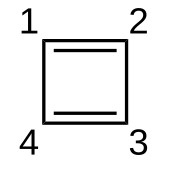
\includegraphics[scale=1.0]{./structures/exercise_1/cyclobutadiene_anion/0.png}
		\captionof{figure}{The order of carbon atoms in the cyclobutadiene anion.}\label{fig:case3}
		\end{center}
		
		For $\pi$-electron atomic orbitals' representation $\Gamma^{\rm AO}$, its following characters is listed below.
		\begin{center}
		\setlength{\abovecaptionskip}{-0.3em}
		\captionof{table}{The character of the $\pi$-electron atomic orbitals' representation $\Gamma^{\rm AO}$.}
		\begin{tabular}{cccccc}\hline
	$\mathscr{D}_{\rm 4}$	& $E$ & $2C_4$ &	$C_2$	& $2C^\prime_2$ & $2C^{\prime\prime}_2$ \\ \hline
	$\chi^{\AO}(C_i)$	&	4	&	0	&	0	&	0	&	-2	\\ \hline
		\end{tabular}
		\end{center}
		
		Relevant reduction coefficients are
		\begin{equation*}
		a_1 = 0, \quad a_2 = 1, \quad b_1 = 1, \quad b_2 = 0, \quad e = 1.
		\end{equation*}
		Then, we arrive at		
		\begin{equation*}
			\Gamma^{\AO} = \Gamma^{A_2} \oplus \Gamma^{B_1} \oplus \Gamma^{E}.
		\end{equation*}
		Thus, to describe the effect of $O_R$, two suitable $2\orbp_{z}$ atomic orbitals is enough. 
		
		Thirdly, we inspect the transformation of $\phi_i$ under $O_R$ for the cyclobutadiene anion, whose information is recorded below. We only list two $\phi_1$ and $\phi_2$.
		\begin{center}
		\setlength{\abovecaptionskip}{-0.5em}
		\captionof{table}{Transformation of $\phi_i$ under $O_R$ for the cyclobutadiene anion.}
		\begin{tabular}{ccccccccc}\hline
	$\mathscr{D}_{\rm 4}$ & $E$ & $C_4$ & $C_2$ & $C^3_4$	&	$C^\prime_{2,1}$	&	$C^\prime_{2,2}$ &	$C^{\prime\prime}_{2,1}$	&	$C^{\prime\prime}_{2,2}$	\\ \hline
			$\phi_1$	&	$\phi_1$	&	$\phi_2$	&	$\phi_3$	&	$\phi_4$	&	$-\phi_2$	&	$-\phi_4$	&	$-\phi_3$	&	$-\phi_1$	\\
			$\phi_2$	&	$\phi_2$	&	$\phi_3$	&	$\phi_4$	&	$\phi_1$	&	$-\phi_1$	&	$-\phi_3$	&	$-\phi_2$	&	$-\phi_4$	\\ \hline
		\end{tabular}
		\end{center}
		
		For the irreducible representation $\Gamma^{A_2}$, the only basis function is
		\begin{align*}
			P^{A_2}\phi_1 &= \sum_{R} \chi^{A_2}(R) O_R \phi_1 = (O_E + O_{C_4} + O_{C_2} + O_{C^3_4} - \sum_{k=1}^2 O_{C^\prime_{2,k}} -\sum_{k=1}^2 O_{C^{\prime\prime}_{2,k}} )\phi_1 \\
			&= 2(\phi_1+\phi_2+\phi_3+\phi_4).
		\end{align*}
		It can be normalized to
		\begin{equation}
			\Phi^\pi_1 = \frac{1}{2}(\phi_1+\phi_2+\phi_3+\phi_4).
		\end{equation}
		
		Then, the effective Hamiltonian for $\pi$ electrons is
		\begin{equation*}
			H^\prime = ( \alpha + 2\beta ).		
		\end{equation*}
		
		In another words, its only eigenvalue is $\alpha + 2\beta$, with eigenfunction $\Phi^\pi_1$.
		
		In conclusion, for the irreducible representation $\Gamma^{A_2}$, relevant results are listed below.
		
		\begin{center}
		\setlength{\abovecaptionskip}{0em}
		\captionof{table}{The H{\"u}ckel MOs in the irreducible representation $\Gamma^{A_2}$ of cyclobutadiene anion.}
		\begin{tabular}{ccc}\hline
		  order	&	eigenvalue		& 	eigenfunction	\\ \hline
			1	&$\alpha+2\beta$& 	$0.5000\phi_1 + 0.5000 \phi_2 + 0.5000 \phi_3 + 0.5000 \phi_4$ \\ \hline
		\end{tabular}
		\end{center}
		
		For the irreducible representation $\Gamma^{B_1}$, the only basis function is
		\begin{align*}
			P^{B_1}\phi_1 &= \sum_{R} \chi^{B_1}(R) O_R \phi_1 = 2(\phi_1 - \phi_2 + \phi_3 - \phi_4).
		\end{align*}
		It can be normalized to
		\begin{equation}
			\Phi^\pi_2 = \frac{1}{2}(\phi_1 - \phi_2 + \phi_3 -\phi_4).
		\end{equation}
		
		Then, the effective Hamiltonian for $\pi$ electrons is
		\begin{equation*}
			H^\prime = ( \alpha - 2\beta ).		
		\end{equation*}
		
		In another words, its only eigenvalue is $\alpha - 2\beta$, with eigenfunction $\Phi^\pi_2$.
		
		In conclusion, for the irreducible representation $\Gamma^{B_1}$, relevant results are listed below.
		
		\begin{center}
		\setlength{\abovecaptionskip}{0em}
		\captionof{table}{The H{\"u}ckel MOs in the irreducible representation $\Gamma^{B_1}$ of cyclobutadiene anion.}
		\begin{tabular}{ccc}\hline
		  order	&	eigenvalue		& 	eigenfunction	\\ \hline
			1	&$\alpha-2\beta$& 	$0.5000\phi_1 - 0.5000 \phi_2 + 0.5000 \phi_3 - 0.5000 \phi_4$ \\ \hline
		\end{tabular}
		\end{center}
		
		For the irreducible representation $\Gamma^{E}$, the only two basis functions are
		\begin{align*}
			P^{E}\phi_1 &= \sum_{R} \chi^{E}(R) O_R \phi_1 = 2(\phi_1 - \phi_3 ), \\
			P^{E}\phi_2 &= \sum_{R} \chi^{E}(R) O_R \phi_2 = 2(\phi_2 - \phi_4 ).	
		\end{align*}
		They can be normalized to
		\begin{align*}
			\phi^\prime_3 &= \frac{1}{\sqrt{2}}(\phi_1 - \phi_3), \\
			\phi^\prime_4 &= \frac{1}{\sqrt{2}}(\phi_2 - \phi_4).
		\end{align*}
		
		Then, the effective Hamiltonian for $\pi$ electrons is
		\begin{equation*}
			H^\prime = \begin{pmatrix}
				\alpha	&	0	\\
				0	&	\alpha
				\end{pmatrix}.				
		\end{equation*}
		It has a two-fold eigenvalue $\alpha$. Thus, corresponding eigenfunctions can be
		\begin{align}
			\Phi^\pi_3 &= \frac{1}{\sqrt{2}}(\phi_1 - \phi_3), \\
			\Phi^\pi_4 &= \frac{1}{\sqrt{2}}(\phi_2 - \phi_4).
		\end{align}
		
		In another words, its only eigenvalue is $\alpha$, with two eigenfunctions $\Phi^\pi_3$ and $\Phi^\pi_4$.
		
		In conclusion, for the irreducible representation $\Gamma^{E}$, relevant results are listed below.
		
		\begin{center}
		\setlength{\abovecaptionskip}{0em}
		\captionof{table}{The H{\"u}ckel MOs in the irreducible representation $\Gamma^{E}$ of cyclobutadiene anion.}
		\begin{tabular}{ccc}\hline
		  order	&	eigenvalue		& 	eigenfunction	\\ \hline
			1	&$\alpha$& 	$0.7071\phi_1 - 0.7071 \phi_3$ \\ 
			2	&$\alpha$& 	$0.7071\phi_2 - 0.7071 \phi_4$ \\\hline
		\end{tabular}
		\end{center}
		
		Now, we have obtained all results, which are shown as following.
		
		\begin{center}
		\setlength{\abovecaptionskip}{-0.5em}
		\captionof{table}{The H{\"u}ckel MOs in all irreducible representations of cyclobutadiene anion.}
		\begin{tabular}{ccccccc}\hline
		order 	& orbital energy & irrep & $c_1$ & $c_2$ & $c_3$ &$c_4$ \\ \hline
			1	&	$\alpha+2.000\beta$	&	$A_2$	&	0.5000	&	0.5000	&	0.5000	&	0.5000	\\
			2	&	$\alpha$	&	$E$	&	0.7071	&	0.0000	&	-0.7071	&	0.0000	\\
			3	&	$\alpha$	&	$E$	&	0.0000	&	0.7071	&	0.0000	&	-0.7071	\\
			4	&	$\alpha-2.000\beta$	&	$B_1$	&	0.5000	&	-0.5000	&	0.5000	&	-0.5000	\\ \hline
		\end{tabular}
		\end{center}
		
		Besides, their phase diagrams have been painted in \Figref{fig:phase_diagram_3}.
		
		\begin{center}
		\begin{tabular}{cccc}
			\begin{minipage}[t]{0.22\linewidth}
			\centering
			\setlength{\abovecaptionskip}{0.5em}
			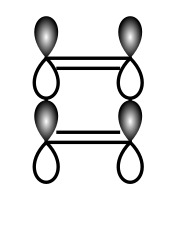
\includegraphics[scale=1]{./structures/exercise_1/cyclobutadiene_anion/1.png}
			\captionof*{figure}{$\varepsilon = \alpha + 2.000\beta$}
			\end{minipage} & 
			\begin{minipage}[t]{0.22\linewidth}
			\setlength{\abovecaptionskip}{0.5em}\hspace*{2em}
			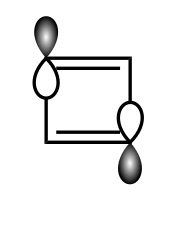
\includegraphics[scale=1]{./structures/exercise_1/cyclobutadiene_anion/3.png}
			\captionof*{figure}{$\varepsilon = \alpha + 0.000\beta$}
			\end{minipage} &
			\begin{minipage}[t]{0.22\linewidth}
			\centering
			\setlength{\abovecaptionskip}{0.5em}
			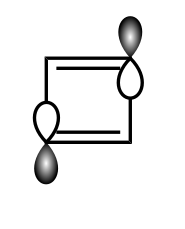
\includegraphics[scale=1]{./structures/exercise_1/cyclobutadiene_anion/4.png}
			\captionof*{figure}{$\varepsilon = \alpha + 0.000\beta$}
			\end{minipage} & 
			\begin{minipage}[t]{0.22\linewidth}
			\setlength{\abovecaptionskip}{0.5em}\hspace{2em}
			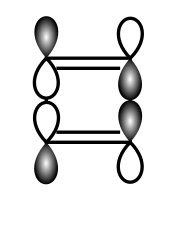
\includegraphics[scale=1]{./structures/exercise_1/cyclobutadiene_anion/2.png}
			\captionof*{figure}{$\varepsilon = \alpha - 2.000\beta$}
			\end{minipage}
		\end{tabular}				
		\captionof{figure}{Phase diagrams of these H{\"u}ckel MOs of cyclobutadiene anion. Black bubbles mean plus phase while white ones mean minus phase. The color is used just for determining relative phase.}\label{fig:phase_diagram_3}
		\end{center}
		
		In the end, we conclude that for cyclobutadiene anion, its ground state $\pi$-electron configuration is $(a_2)^2(e)^4$ and its delocalization energy is $-2.000\beta$, which means that cyclobutadiene anion needs other stable structures to stabilize itself.
		
		
		\item Firstly, it is easy find that cyclopentadienyl radical belongs to the point group $\mathscr{D}_{\rm 5h}$. However, it has only 5 $\pi$-electrons. Just $\mathscr{D}_{\rm 5}$ is good enough and its character table is shown in \Tableref{tab:chatab_3}.
		\begin{center}
		\setlength{\abovecaptionskip}{0em}
		\captionof{table}{The character table for the $\mathscr{D}_{\rm 5}$ point group. Here, $\gamma = \frac{2\pi}{5}$.}\label{tab:chatab_4}
		\begin{tabular}{ccccc}\hline
	$\mathscr{D}_{\rm 5}$ & $E$ & $2C_5$ &	$2C^2_5$	& $5C^\prime_2$ \\ \hline
			$A_1$	&	1	&	1	&	1	&	1	\\
			$A_2$	&	1	&	1	&	1	&	-1	\\
			$E_1$ 	&	2	&$2\cos\gamma$	&	$2\cos2\gamma$	&	0	\\
			$E_2$ 	&	2	&$2\cos2\gamma$	&	$2\cos\gamma$	&	0	\\ \hline
		\end{tabular}
		\end{center}
		
		Secondly, we mark all carbon atoms as follows.
		\begin{center}
		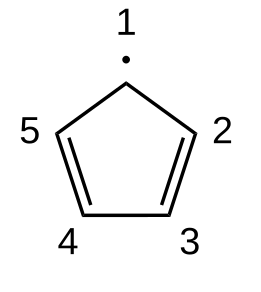
\includegraphics[scale=1.0]{./structures/exercise_1/cyclopentadienyl_radical/0.png}
		\setlength{\abovecaptionskip}{-0.3em}
		\captionof{figure}{The order of carbon atoms in cyclopentadienyl radical.}
		\setlength{\belowcaptionskip}{-0.8em}
		\end{center}				

		For $\pi$-electron atomic orbitals' representation $\Gamma^{\rm AO}$, its following characters is listed below.
		\begin{center}
		\setlength{\abovecaptionskip}{-0.3em}
		\captionof{table}{The character of the $\pi$-electron atomic orbitals' representation $\Gamma^{\rm AO}$.}
		\begin{tabular}{ccccc}\hline
	$\mathscr{D}_{\rm 5}$	& $E$ & $2C_5$ &	$2C^2_5$	& $5C^\prime_2$ \\ \hline
	$\chi^{\AO}(C_i)$	&	5	&	0	&	0	&	-1	\\ \hline
		\end{tabular}\vspace*{-0.5em}
		\end{center}
		Relevant reduction coefficients are
		\begin{equation*}
		a_1 = 0, \quad a_2 = 1, \quad e_1 = 1, \quad e_2 = 1,
		\end{equation*}
		which equal to
		\begin{equation*}
			\Gamma^{\AO} = \Gamma^{A_2} \oplus \Gamma^{E_1} \oplus \Gamma^{E_2}.
		\end{equation*}
		
		\begin{center}
		\begin{tabular}{ccccccccccc}\hline
	$\mathscr{D}_{\rm 5}$ & $E$ & $C^1_5$ & $C^2_5$ & $C^3_5$	&	$C^4_5$	&	$C^\prime_{2,1}$	&	$C^\prime_{2,2}$ &	$C^\prime_{2,3}$	&	$C^\prime_{2,4}$	&	$C^\prime_{2,5}$	\\ \hline
			$\phi_1$	&	$\phi_1$	&	$\phi_2$	&	$\phi_3$	&	$\phi_4$	&	$\phi_5$	&	$-\phi_1$	&	$-\phi_3$	&	$-\phi_5$	&	$-\phi_2$	&	$-\phi_4$	\\
			$\phi_2$	&	$\phi_2$	&	$\phi_3$	&	$\phi_4$	&	$\phi_5$	&	$\phi_1$	&	$-\phi_5$	&	$-\phi_2$	&	$-\phi_4$	&	$-\phi_1$	&	$-\phi_3$	\\ \hline
		\end{tabular}
		\end{center}
		
		For the irreducible representation $\Gamma^{A_2}$, the only basis function is
		\begin{align*}
			P^{A_2}\phi_1 &= \sum_{R} \chi^{A_2}(R) O_R \phi_1 = 2(\phi_1 + \phi_2 + \phi_3 + \phi_4 + \phi_5).
		\end{align*}
		It can be normalized to
		\begin{equation}
			\phi^\prime_1 = \frac{1}{\sqrt{5}}(\phi_1 + \phi_2 + \phi_3 + \phi_4 + \phi_5).
		\end{equation}
		
		Then, the effective Hamiltonian for $\pi$ electrons is
		\begin{equation*}
			H^\prime = ( \alpha + 2\beta ).		
		\end{equation*}
		
		In another words, its only eigenvalue is $\alpha + 2\beta$, with eigenfunction $\Phi^\pi_1 = \phi^\prime_1$.
		
		In conclusion, for the irreducible representation $\Gamma^{A_2}$, relevant results are listed below.
		
		\begin{center}
		\setlength{\abovecaptionskip}{0em}
		\captionof{table}{The H{\"u}ckel MOs in the irreducible representation $\Gamma^{A_2}$ of cyclopentadienyl radical.}
		\begin{tabular}{ccc}\hline
		  order	&	eigenvalue		& 	eigenfunction	\\ \hline
			1	&$\alpha+2\beta$& 	$0.4472\phi_1 + 0.4472 \phi_2 + 0.4472 \phi_3 + 0.4472 \phi_4 + 0.4472 \phi_5$ \\ \hline
		\end{tabular}
		\end{center}
		
		For the irreducible representation $\Gamma^{E_1}$, the only two basis functions are
		\begin{align*}
			P^{E_1}\phi_1 &= \sum_{R} \chi^{E_1}(R) O_R \phi_1 = 2\phi_1 + \frac{\sqrt{5}-1}{2}(\phi_2 + \phi_5) - \frac{\sqrt{5}+1}{2}(\phi_3 + \phi_4). \\
			P^{E_1}\phi_2 &= \sum_{R} \chi^{E_1}(R) O_R \phi_2 = 2\phi_2 + \frac{\sqrt{5}-1}{2}(\phi_1 + \phi_3) - \frac{\sqrt{5}+1}{2}(\phi_4 + \phi_5).
		\end{align*}
		They can be normalized to
		\begin{align*}
			\phi^\prime_2 &= \sqrt{\frac{1}{10}} P^{E_1}\phi_1 = \sqrt{ \frac{2}{5} }\phi_1 + \frac{\sqrt{5}-1}{2\sqrt{10}}(\phi_2+\phi_5) - \frac{\sqrt{5}+1}{2\sqrt{10}}(\phi_3+\phi_4) \\
			&= \sqrt{ \frac{2}{5} } \left[ \phi_1 + \phi_2 \cos\gamma + \phi_3\cos2\gamma + \phi_4\cos2\gamma + \phi_5\cos\gamma \right], \\
			\phi^\prime_3 &= \sqrt{\frac{1}{10}} P^{E_1}\phi_2 = \sqrt{ \frac{2}{5} }\phi_2 + \frac{\sqrt{5}-1}{2\sqrt{10}}(\phi_1+\phi_3) - \frac{\sqrt{5}+1}{2\sqrt{10}}(\phi_4+\phi_5) \\
			&= \sqrt{ \frac{2}{5} } \left[ \phi_1\cos\gamma + \phi_2  + \phi_3\cos\gamma + \phi_4\cos2\gamma + \phi_5\cos2\gamma \right].
		\end{align*}
		However, they are not mutually orthogonal! We have to orthogonalize $\phi^\prime_2$ and $\phi^\prime_3$,
		\begin{align*}
			\phi^\prime_2 + \phi^\prime_3 &= \sqrt{ \frac{2}{5} } \left[ (\phi_1+\phi_2) (1+\cos\gamma) + (\phi_3+\phi_5) (\cos\gamma + \cos 2\gamma) + 2\phi_4\cos2\gamma \right] \\
			&= \sqrt{ \frac{2}{5} } \left[ \frac{3+\sqrt{5}}{4}(\phi_1 + \phi_2) - \frac{1}{2} (\phi_3 + \phi_5) - \frac{ \sqrt{5}+1 }{2} \Phi_4 \right] , \\
			\phi^\prime_2 - \phi^\prime_3 &= \sqrt{ \frac{2}{5} } \left[ (\phi_1-\phi_2) (1-\cos\gamma) + (\phi_3-\phi_5) (\cos2\gamma - \cos\gamma) \right] \\
			&=\sqrt{ \frac{2}{5} } \left[ \frac{ 5-\sqrt{5} }{4} (\phi_1 - \phi_2) - \frac{ \sqrt{5} }{2} (\phi_3 - \phi_5) \right].
		\end{align*}
		and then normalize them. Their sum of squares of coefficients are
		\begin{align*}
			\sum_{k=1}^5 c^2_{2,k} &= \frac{3+\sqrt{5}}{2}, \\
			\sum_{k=1}^5 c^2_{3,k} &= \frac{5-\sqrt{5}}{2},
		\end{align*}
		and then
		\begin{align*}
			\phi^{\prime\prime}_2 &= \sqrt{ \frac{2}{3+\sqrt{5}} } \left[ \phi^\prime_2 + \phi^\prime_3 \right] = \frac{2}{ \sqrt{5(3+\sqrt{5})} } \left[ \frac{3+\sqrt{5}}{4}(\phi_1 + \phi_2) - \frac{1}{2} (\phi_3 + \phi_5) - \frac{ \sqrt{5}+1 }{2} \Phi_4 \right]\\
			&= \frac{ \sqrt{3+\sqrt{5}} }{2\sqrt{5}}(\phi_1 + \phi_2) - \frac{1}{ \sqrt{ 5(3+\sqrt{5}) } } (\phi_3 + \phi_5) - \frac{ 1+\sqrt{5} }{ \sqrt{ 5(3+\sqrt{5}) } } \phi_4 \\
			&\approx 0.5117 \phi_1 + 0.5117 \phi_2 -0.1954 \phi_3 -0.6325\phi_4 -0.1954 \phi_5 , \\
			\phi^{\prime\prime}_3 &= \sqrt{ \frac{2}{5-\sqrt{5}} } \left[ \phi^\prime_2 - \phi^\prime_3 \right] = \frac{2}{ \sqrt{5(5-\sqrt{5})} }\left[ \frac{ 5-\sqrt{5} }{4} (\phi_1 - \phi_2) - \frac{ \sqrt{5} }{2} (\phi_3 - \phi_5) \right] \\
			&= \frac{ \sqrt{ 5-\sqrt{5} } }{ 2\sqrt{5} } (\phi_1 - \phi_2) - \frac{ 1 }{ \sqrt{ 5-\sqrt{5} } }(\phi_3 - \phi_5) \\
			&\approx 0.3717 \phi_1 - 0.3717 \phi_2 - 0.6015\phi_3 + 0.6015 \phi_5.
		\end{align*}
		
		Then, the effective Hamiltonian for $\pi$ electrons is
		\begin{equation*}
			H^\prime = \begin{pmatrix}
				\alpha + \frac{ \sqrt{5}-1 }{2}\beta & 0 \\
				0 & \alpha + \frac{ \sqrt{5}-1 }{2}\beta
			\end{pmatrix} \approx
			\begin{pmatrix}
				\alpha + 0.618 \beta & 0 \\ 0 & \alpha + 0.618 \beta
			\end{pmatrix}				,
		\end{equation*}
		
		In another words, it has only one two-fold eigenvalue $\alpha + \frac{ \sqrt{5}-1 }{2} \beta\approx \alpha + 0.618 \beta$, with two mutually orthogonal eigenfunctions $\Phi^\pi_2 = \phi^{\prime\prime}_2$, $\Phi^\pi_3 = \phi^{\prime\prime}_3$.
		
		In conclusion, for the irreducible representation $\Gamma^{E_1}$, relevant results are listed below.
		
		\begin{center}
		\setlength{\abovecaptionskip}{0em}
		\captionof{table}{The H{\"u}ckel MOs in the irreducible representation $\Gamma^{E_1}$ of cyclopentadienyl radical.}
		\begin{tabular}{ccc}\hline
		  order	&	eigenvalue		& 	eigenfunction	\\ \hline
			1	&$\alpha+0.618\beta$& 	$0.5117\phi_1 + 0.5117 \phi_2 -0.1954 \phi_3 -0.6325 \phi_4 -0.1954 \phi_5$ \\
			2	&$\alpha+0.618\beta$& 	$0.3717\phi_1 - 0.3717 \phi_2 -0.6015 \phi_3 +0.0000 \phi_4 +0.6015 \phi_5$ \\
			 \hline
		\end{tabular}
		\end{center}
		
		For the irreducible representation $\Gamma^{E_2}$, the only two basis functions are
		\begin{align*}
			P^{E_2}\phi_1 &= \sum_{R} \chi^{E_2}(R) O_R \phi_1 = 2\phi_1 - \frac{\sqrt{5}+1}{2}(\phi_2 + \phi_5) + \frac{\sqrt{5}-1}{2}(\phi_3 + \phi_4). \\
			P^{E_2}\phi_2 &= \sum_{R} \chi^{E_2}(R) O_R \phi_2 = 2\phi_2 - \frac{\sqrt{5}+1}{2}(\phi_1 + \phi_3) + \frac{\sqrt{5}-1}{2}(\phi_4 + \phi_5).
		\end{align*}
		They can be normalized to
		\begin{align*}
			\phi^\prime_4 &= \sqrt{\frac{1}{10}} P^{E_1}\phi_1 = \sqrt{ \frac{2}{5} }\phi_1 - \frac{\sqrt{5}+1}{2\sqrt{10}}(\phi_2+\phi_5) + \frac{\sqrt{5}-1}{2\sqrt{10}}(\phi_3+\phi_4) \\
			&= \sqrt{ \frac{2}{5} } \left[ \phi_1 + \phi_2 \cos2\gamma + \phi_3\cos\gamma + \phi_4\cos\gamma + \phi_5\cos2\gamma \right], \\
			\phi^\prime_5 &= \sqrt{\frac{1}{10}} P^{E_1}\phi_2 = \sqrt{ \frac{2}{5} }\phi_2 - \frac{\sqrt{5}+1}{2\sqrt{10}}(\phi_1+\phi_3) - \frac{\sqrt{5}-1}{2\sqrt{10}}(\phi_4+\phi_5) \\
			&= \sqrt{ \frac{2}{5} } \left[ \phi_1\cos2\gamma + \phi_2  + \phi_3\cos2\gamma + \phi_4\cos\gamma + \phi_5\cos\gamma \right].
		\end{align*}
		However, they are not mutually orthogonal! We have to orthogonalize $\phi^\prime_4$ and $\phi^\prime_5$,
		\begin{align*}
			\phi^\prime_4 + \phi^\prime_5 &= \sqrt{ \frac{2}{5} } \left[ (\phi_1+\phi_2) (1+\cos2\gamma) + (\phi_3+\phi_5) (\cos\gamma + \cos 2\gamma) + 2\phi_4\cos\gamma \right] \\
			&= \sqrt{ \frac{2}{5} } \left[ \frac{3-\sqrt{5}}{4}(\phi_1 + \phi_2) - \frac{1}{2} (\phi_3 + \phi_5) + \frac{ \sqrt{5}-1 }{2} \Phi_4 \right] , \\
			\phi^\prime_4 - \phi^\prime_5 &= \sqrt{ \frac{2}{5} } \left[ (\phi_1-\phi_2) (1-\cos2\gamma) + (\phi_3-\phi_5) (\cos\gamma - \cos2\gamma) \right] \\
			&=\sqrt{ \frac{2}{5} } \left[ \frac{ 5+\sqrt{5} }{4} (\phi_1 - \phi_2) + \frac{ \sqrt{5} }{2} (\phi_3 - \phi_5) \right].
		\end{align*}
		and then normalize them. Their sum of squares of coefficients are
		\begin{align*}
			\sum_{k=1}^5 c^2_{4,k} &= \frac{3-\sqrt{5}}{2}, \\
			\sum_{k=1}^5 c^2_{5,k} &= \frac{5+\sqrt{5}}{2},
		\end{align*}
		and then
		\begin{align*}
			\phi^{\prime\prime}_4 &= \sqrt{ \frac{2}{3-\sqrt{5}} } \left[ \phi^\prime_4 + \phi^\prime_5 \right] = \frac{2}{ \sqrt{5(3-\sqrt{5})} } \left[ \frac{3-\sqrt{5}}{4}(\phi_1 + \phi_2) - \frac{1}{2} (\phi_3 + \phi_5) + \frac{ \sqrt{5}-1 }{2} \Phi_4 \right]\\
			&= \frac{ \sqrt{3-\sqrt{5}} }{2\sqrt{5}}(\phi_1 + \phi_2) - \frac{1}{ \sqrt{ 5(3-\sqrt{5}) } } (\phi_3 + \phi_5) + \frac{ \sqrt{5}-1 }{ \sqrt{ 5(3-\sqrt{5}) } } \phi_4 \\
			&\approx 0.1954 \phi_1 + 0.1954 \phi_2 - 0.5117 \phi_3 +0.6325\phi_4 -0.5117 \phi_5 , \\
			\phi^{\prime\prime}_5 &= \sqrt{ \frac{2}{5+\sqrt{5}} } \left[ \phi^\prime_4 - \phi^\prime_5 \right] = \frac{2}{ \sqrt{5(5+\sqrt{5})} }\left[ \frac{ 5+\sqrt{5} }{4} (\phi_1 - \phi_2) + \frac{ \sqrt{5} }{2} (\phi_3 - \phi_5) \right] \\
			&= \frac{ \sqrt{ 5+\sqrt{5} } }{ 2\sqrt{5} } (\phi_1 - \phi_2) + \frac{ 1 }{ \sqrt{ 5+\sqrt{5} } }(\phi_3 - \phi_5) \\
			&\approx 0.6015 \phi_1 - 0.6015 \phi_2 + 0.3717\phi_3 -0.3717 \phi_5.
		\end{align*}
		
		Then, the effective Hamiltonian for $\pi$ electrons is
		\begin{equation*}
			H^\prime = \begin{pmatrix}
				\alpha - \frac{ \sqrt{5}+1 }{2}\beta & 0 \\
				0 & \alpha - \frac{ \sqrt{5}+1 }{2}\beta
			\end{pmatrix} \approx
			\begin{pmatrix}
				\alpha - 1.618 \beta & 0 \\ 0 & \alpha - 1.618 \beta
			\end{pmatrix}				,
		\end{equation*}
		
		In another words, it has only one two-fold eigenvalue $\alpha + \frac{ \sqrt{5}-1 }{2} \beta\approx \alpha - 1.618 \beta$, with two mutually orthogonal eigenfunctions $\Phi^\pi_4 = \phi^{\prime\prime}_4$, $\Phi^\pi_5 = \phi^{\prime\prime}_5$.
		
		In conclusion, for the irreducible representation $\Gamma^{E_2}$, relevant results are listed below.
		
		\begin{center}
		\setlength{\abovecaptionskip}{0em}
		\captionof{table}{The H{\"u}ckel MOs in the irreducible representation $\Gamma^{E_2}$ of cyclopentadienyl radical.}
		\begin{tabular}{ccc}\hline
		  order	&	eigenvalue		& 	eigenfunction	\\ \hline
			1	&$\alpha-1.618\beta$& 	$0.1954\phi_1 + 0.1954 \phi_2 -0.5117 \phi_3 +0.6325 \phi_4 -0.5117 \phi_5$ \\
			2	&$\alpha-1.618\beta$& 	$0.6015\phi_1 - 0.6015 \phi_2 +0.3717 \phi_3 +0.0000 \phi_4 -0.3717 \phi_5$ \\	 \hline
		\end{tabular}
		\end{center}
		
		Now, we have obtained all results, which are shown as following.
		
		\begin{center}
		\setlength{\abovecaptionskip}{-0.5em}
		\captionof{table}{The H{\"u}ckel MOs in all irreducible representations of cyclopentadienyl radical.}
		\begin{tabular}{cccccccc}\hline
		order 	& orbital energy & irrep & $c_1$ & $c_2$ & $c_3$ &$c_4$ &	$c_5$	\\ \hline
			1	&	$\alpha+2.000\beta$	&	$A_2$	&	0.4472	&	0.4472	&	0.4472	&	0.4472	&	0.4472	\\
			2	&	$\alpha+0.618\beta$	&	$E_1$	&	0.5117	&	0.5117	&	-0.1954	&	-0.6325	&	-0.1954	\\
			3	&	$\alpha+0.618\beta$	&	$E_1$	&	0.3717	&	-0.3717	&	-0.6015	&	0.0000	&	0.6015	\\
			4	&	$\alpha-1.618\beta$	&	$E_2$	&	0.1954	&	0.1954	&	-0.5117	&	0.6325	&	-0.5117	\\
			5	&	$\alpha-1.618\beta$	&	$E_2$	&	0.6015	&	-0.6015	&	0.3717	&	0.0000	&	-0.3717	\\ \hline
		\end{tabular}
		\end{center}
		
		Besides, their phase diagrams have been painted in \Figref{fig:phase_diagram_4}.
		
		\begin{center}
		\begin{tabular}{ccccc}
			\begin{minipage}[t]{0.17\linewidth}
			\centering
			\setlength{\abovecaptionskip}{0.5em}
			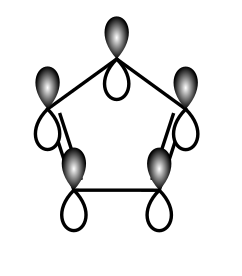
\includegraphics[scale=1]{./structures/exercise_1/cyclopentadienyl_radical/1.png}
			\captionof*{figure}{$\varepsilon = \alpha + 2.000\beta$}
			\end{minipage} & 
			\begin{minipage}[t]{0.17\linewidth}
			\setlength{\abovecaptionskip}{0.5em}\hspace*{0.2em}
			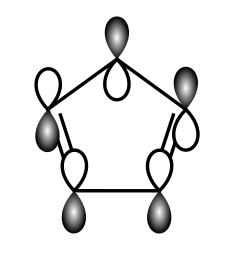
\includegraphics[scale=1]{./structures/exercise_1/cyclopentadienyl_radical/2.png}
			\captionof*{figure}{$\varepsilon = \alpha + 0.618\beta$}
			\end{minipage} &
			\begin{minipage}[t]{0.18\linewidth}
			\centering
			\setlength{\abovecaptionskip}{0.5em}
			\hspace*{-0.2em}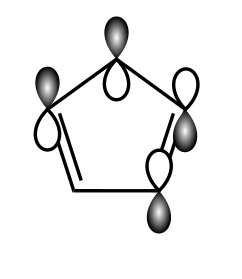
\includegraphics[scale=1]{./structures/exercise_1/cyclopentadienyl_radical/3.png}
			\captionof*{figure}{$\varepsilon = \alpha + 0.000\beta$}
			\end{minipage} & 
			\begin{minipage}[t]{0.18\linewidth}
			\setlength{\abovecaptionskip}{0.5em}\hspace*{0.5em}
			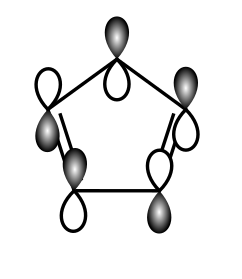
\includegraphics[scale=1]{./structures/exercise_1/cyclopentadienyl_radical/4.png}
			\captionof*{figure}{$\varepsilon = \alpha - 2.000\beta$}
			\end{minipage}
			\begin{minipage}[t]{0.18\linewidth}
			\setlength{\abovecaptionskip}{0.5em}\hspace*{0.5em}
			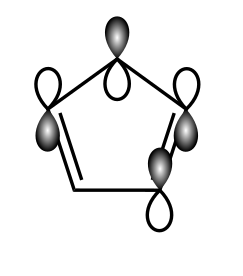
\includegraphics[scale=1]{./structures/exercise_1/cyclopentadienyl_radical/5.png}
			\captionof*{figure}{$\varepsilon = \alpha - 2.000\beta$}
			\end{minipage}
		\end{tabular}				
		\captionof{figure}{Phase diagrams of these H{\"u}ckel MOs of cyclopentadienyl radical. Black bubbles mean plus phase while white ones mean minus phase. The color is used just for determining relative phase.}\label{fig:phase_diagram_4}
		\end{center}
		
		In the end, we conclude that for cyclopentadienyl radical, its ground state $\pi$-electron configuration is $(a_2)^2(e_1)^3$ and its delocalization energy is $2 \times 2.000 \beta + 3 \times 0.618 \beta - 5 \times 1.000 \beta = 0.854 \beta$, much larger than {\it trans}-1,3-butadiene ($0.472\beta$) but also much smaller than benzene ($2.000\beta$). 
		
		\item 5555555555555555   naphthalene
		
		Firstly, it is easy find that naphthalene belongs to the point group $\mathscr{D}_{\rm 2h}$, whose character table is shown in \Tableref{tab:chatab_5}.		
		\begin{center}
		\setlength{\abovecaptionskip}{0em}
		\captionof{table}{The character table for the $\mathscr{D}_{\rm 2h}$ point group.}\label{tab:chatab_5}
		\begin{tabular}{ccccccccc}\hline
	$\mathscr{D}_{\rm 2h}$ & $E$ & $C_{2z}$ &	$C_{2y}$	& $C_{2x}$	&	$i$	&	$\sigma_{xy}$	&	$\sigma_{xz}$ &	$\sigma_{yz}$\\ \hline
			$A_g$		&	1	&	1	&	1	&	1	&	1	&	1	&	1	&	1	\\
			$B_{1g}$	&	1	&	1	&	-1	&	-1	&	1	&	1	&	-1	&	-1	\\
			$B_{2g}$ 	&	1	&	-1	&	1	&	-1	&	1	&	-1	&	1	&	-1	\\
			$B_{3g}$ 	&	1	&	-1	&	-1	&	1	&	1	&	-1	&	-1	&	1	\\ 
			$A_u$		&	1	&	1	&	1	&	1	&	-1	&	-1	&	-1	&	-1	\\
			$B_{1u}$	&	1	&	1	&	-1	&	-1	&	-1	&	-1	&	1	&	1	\\
			$B_{2u}$ 	&	1	&	-1	&	1	&	-1	&	-1	&	1	&	-1	&	1	\\
			$B_{3u}$ 	&	1	&	-1	&	-1	&	1	&	-1	&	1	&	1	&	-1	\\ \hline
		\end{tabular}
		\end{center}
		
		Secondly, we mark all carbon atoms as follows.
		\begin{center}
		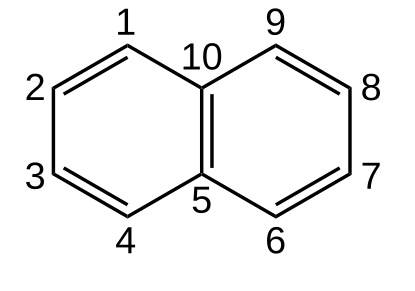
\includegraphics[scale=1.0]{./structures/exercise_1/naphthalene/0.png}
		\setlength{\abovecaptionskip}{-0.3em}
		\captionof{figure}{The order of carbon atoms in naphthalene.}
		\setlength{\belowcaptionskip}{-0.8em}
		\end{center}	
		
		For $\pi$-electron atomic orbitals' representation $\Gamma^{\rm AO}$, its following characters is listed below.		
		\begin{center}
		\setlength{\abovecaptionskip}{-0.3em}
		\captionof{table}{The character of the $\pi$-electron atomic orbitals' representation $\Gamma^{\rm AO}$.}
		\begin{tabular}{ccccccccc}\hline
	$\mathscr{D}_{\rm 2h}$	& $E$ & $C_{2z}$ &	$C_{2y}$	& $C_{2x}$	&	$i$	$\sigma_{xy}$	&	$\sigma_{xz}$	&	$\sigma_{xz}$ &	$\sigma_{yz}$  \\ \hline
	$\chi^{\AO}(C_i)$	&	10	&	0	&	-2	&	0	&	0	&	-10	&	0	&	2	\\ \hline
		\end{tabular}\vspace*{-0.5em}
		\end{center}
		Relevant reduction coefficients are
		\begin{align*}
			a_g = 0,	\quad	b_{1g} = 0,	\quad	b_{2g} = 2,	\quad	b_{3g} = 3,	\quad a_u = 2,	\quad b_{1u} = 3,	\quad	b_{2u} = 0,	\quad	b_{3u} = 0.
		\end{align*}
		Thus, we arrive at
		\begin{equation*}
			\Gamma^{\AO} = 2\Gamma^{B_{2g}} \oplus 3\Gamma^{B_{3g}} \oplus 2\Gamma^{A_u} \oplus 3\Gamma^{B_{1u}}.
		\end{equation*}
		We conclude that there are three basis functions in the irreducible representation $\Gamma^{B_{3g}}$ and $\Gamma^{B_{1u}}$, respectively. Thus, to describe the effect of $O_R$, three suitable $2 \orbp_z$ atomic orbitals $\phi_i$ is enough.
		
		\begin{center}
		\setlength{\abovecaptionskip}{0em}
		\captionof{table}{Transformation of $\phi_i$ under $O_R$ for the naphthalene.}
		\begin{tabular}{ccccccccc}\hline
	$\mathscr{D}_{\rm 5}$ & $E$ & $C_{2z}$ & $C_{2y}$ & $C_{2x}$	&	$i$	&	$\sigma_{xy}$ &	$\sigma_{xz}$	&	$\sigma_{yz}$\\ \hline
			$\phi_1$	&	$\phi_1$	&	$\phi_6$	&	$-\phi_9$	&	$-\phi_4$	&	$-\phi_6$	&	$-\phi_1$	&	$\phi_4$	&	$\phi_9$		\\
			$\phi_2$	&	$\phi_2$	&	$\phi_7$	&	$-\phi_8$	&	$-\phi_3$	&	$-\phi_7$	&	$-\phi_2$	&	$\phi_3$	&	$\phi_8$		\\ 
			$\phi_5$	&	$\phi_5$	&	$\phi_{10}$	&	$-\phi_5$	&	$-\phi_{10}$	&	$-\phi_{10}$	&	$-\phi_5$	&	$\phi_{10}$	&	$\phi_5$		\\\hline
		\end{tabular}
		\end{center}
		
		For the irreducible representation $\Gamma^{B_{2g}}$, the only two basis functions are
		\begin{align*}
			P^{B_{2g}}\phi_1 &= \sum_{R} \chi^{B_{2g}}(R) O_R \phi_1 = 2(\phi_1 + \phi_4 - \phi_6 - \phi_9 ), \\
			P^{B_{2g}}\phi_2 &= \sum_{R} \chi^{B_{2g}}(R) O_R \phi_2 = 2(\phi_2 + \phi_3 - \phi_7 - \phi_8 ).	
		\end{align*}
		They can be normalized to
		\begin{align*}
			\phi^\prime_1 &= \frac{1}{2}(\phi_1 + \phi_4 - \phi_6 - \phi_9), \\
			\phi^\prime_2 &= \frac{1}{2}(\phi_2 + \phi_3 - \phi_7 - \phi_8).
		\end{align*}
		Besides, it is easy to find that they are mutually orthogonal.
		
		Then, the effective Hamiltonian for $\pi$ electrons is
		\begin{equation*}
			H^\prime_{B_{2g}} = \begin{pmatrix}
				\alpha	&	\beta	\\
				\beta	&	\alpha+\beta
				\end{pmatrix}.				
		\end{equation*}
		Its eigen equation is		
		\begin{equation}
			\det(\Hp_{B_{2g}}-\varepsilon^\pi \Sp_{B_{2g}}) = \beta^2 ( x^2 + x - 1 ) = 0.
		\end{equation}
		There are two roots,
		\begin{equation}
			x_1 = \frac{-1+\sqrt{5}}{2}, \quad x_2 = \frac{-1-\sqrt{5}}{2},
		\end{equation}
		which equal to
		\begin{align}
			\varepsilon^\pi_1 &= \alpha - \frac{\sqrt{5}-1}{2}\beta, \\
			\varepsilon^\pi_2 &= \alpha + \frac{\sqrt{5}+1}{2}\beta.
		\end{align}
		
		For $\Hp_{B_{2g}}-\varepsilon^\pi_1 \Sp_{B_{2g}}$, its reduced row echelon form is
		\begin{equation*}
			\begin{pmatrix}
				1	& \frac{1+\sqrt{5}}{2}	\\	0	&	0
			\end{pmatrix},
		\end{equation*}
		which means
		\begin{equation*}
			\Phi_1 = \frac{\sqrt{5}+1}{2}\phi^\prime_1 - \phi^\prime_2.
		\end{equation*}
		The sum of squares of coefficients is
		\begin{equation*}
			\sum_{i} c^2_i = \frac{ 5+\sqrt{5} }{2},
		\end{equation*}
		Thus, we know
		\begin{align}
			\Phi^\pi_1 &= \sqrt{ \frac{2}{5+\sqrt{5}} } \Phi_1 = \sqrt{ \frac{2}{5+\sqrt{5}} } \left[ \frac{\sqrt{5}+1}{2}\phi^\prime_1 - \phi^\prime_2 \right] = \sqrt{\frac{\sqrt{5}+1}{2\sqrt{5}}} \phi^\prime_1 - \sqrt{\frac{\sqrt{5}-1}{2\sqrt{5}}} \phi^\prime_2	\notag \\
			&= \frac{1}{2}\sqrt{\frac{\sqrt{5}+1}{2\sqrt{5}}} (\phi_1 + \phi_4 - \phi_6 - \phi_9) - \frac 12 \sqrt{\frac{\sqrt{5}-1}{2\sqrt{5}}} (\phi_2 + \phi_3 - \phi_7 - \phi_8)\notag \\
			&\approx 0.4253 \phi_1 - 0.2629 \phi_2 - 0.2629 \phi_3 + 0.4253 \phi_4 - 0.4253\phi_6 + 0.2629\phi_7 + 0.2629\phi_8 - 0.4253 \phi_9.
		\end{align}
		
		Similarly, the reduced row echelon form of $\Hp_{B_{2g}}-\varepsilon^\pi_2 \Sp_{B_{2g}}$ is
		\begin{equation*}
			\begin{pmatrix}
				1	& \frac{1-\sqrt{5}}{2}	\\	0	&	0
			\end{pmatrix},
		\end{equation*}		
		which means
		\begin{equation*}
			\Phi_2 = \frac{\sqrt{5}-1}{2}\phi^\prime_1 + \phi^\prime_2.
		\end{equation*}
		And then,
		\begin{align}
			\Phi^\pi_2 &= \sqrt{ \frac{2}{5-\sqrt{5}} } \Phi_2 = \sqrt{\frac{\sqrt{5}-1}{2\sqrt{5}}} \phi^\prime_1 + \sqrt{\frac{\sqrt{5}+1}{2\sqrt{5}}} \phi^\prime_2	\notag \\
			&= \frac{1}{2}\sqrt{\frac{\sqrt{5}+1}{2\sqrt{5}}}(\phi_1 + \phi_4 - \phi_6 - \phi_9) + \frac{1}{2}\sqrt{\frac{\sqrt{5}-1}{2\sqrt{5}}} (\phi_2 + \phi_3 - \phi_7 - \phi_8) \notag \\
			&\approx 0.2629 \phi_1 + 0.4253 \phi_2 + 0.4253 \phi_3 + 0.2629 \phi_4 - 0.2629\phi_6 - 0.4253 \phi_7 - 0.4253 \phi_8 - 0.2629 \phi_9.
		\end{align}

		In conclusion, for the irreducible representation $\Gamma^{B_{2g}}$, relevant results are listed below.
		
		\begin{center}
		\setlength{\abovecaptionskip}{0em}
		\captionof{table}{The H{\"u}ckel MOs in the irreducible representation $\Gamma^{B_{2g}}$ of naphthalene.}
		\begin{tabular}{ccccccc}\hline
		order & eigenvalue & \multicolumn{5}{c}{eigenfunction} \\ \hline
		\multirow{4}*{1}	&	\multirow{4}*{$\alpha-0.618\beta$}	&	$c_1$	&	$c_2$	&	$c_3$	&	$c_4$	&	$c_5$	\\	\cline{3-7}
			&	&	0.4253 &	- 0.2629	&	- 0.2629	&	0.4253	&	0.0000	\\	\cline{3-7}
			&	&	$c_6$	&	$c_7$	&	$c_8$	&	$c_9$	&	$c_{10}$	\\	\cline{3-7}
			&	&	- 0.4253	&	0.2629	&	0.2629	&	- 0.4253	&	0.0000	\\	\hline
		\multirow{4}*{2}	&	\multirow{4}*{$\alpha+1.618\beta$}	&	$c_1$	&	$c_2$	&	$c_3$	&	$c_4$	&	$c_5$	\\	\cline{3-7}
			&	&	0.2629 &	0.4253	&	0.4253	&	0.2629	&	0.0000	\\	\cline{3-7}
			&	&	$c_6$	&	$c_7$	&	$c_8$	&	$c_9$	&	$c_{10}$	\\	\cline{3-7}
			&	&	- 0.2629	&	-0.4253	&	- 0.4253	&	-0.2629	&	0.0000	\\	\hline
		\end{tabular}
		\end{center}
		
		For the irreducible representation $\Gamma^{B_{3g}}$, the only three basis functions are
		\begin{align*}
			P^{B_{3g}}\phi_1 &= \sum_{R} \chi^{B_{3g}}(R) O_R \phi_1 = 2(\phi_1 - \phi_4 - \phi_6 + \phi_9 ), \\
			P^{B_{3g}}\phi_2 &= \sum_{R} \chi^{B_{3g}}(R) O_R \phi_2 = 2(\phi_2 - \phi_3 - \phi_7 + \phi_8 ),  \\
			P^{B_{3g}}\phi_5 &= \sum_{R} \chi^{B_{3g}}(R) O_R \phi_5 = 4(\phi_5- \phi_{10} ).
		\end{align*}
		They can be normalized to
		\begin{align*}
			\phi^\prime_3 &= \frac{1}{2}(\phi_1 - \phi_4 - \phi_6 + \phi_9), \\
			\phi^\prime_4 &= \frac{1}{2}(\phi_2 - \phi_3 - \phi_7 + \phi_8), \\
			\phi^\prime_5 &= \frac{1}{\sqrt{2}}(\phi_5 - \phi_{10}).
		\end{align*}
		Besides, it is easy to find that they are mutually orthogonal.
		
		Then, the effective Hamiltonian for $\pi$ electrons is
		\begin{equation*}
			H^\prime_{B_{3g}} = \begin{pmatrix}
				\alpha	&	\beta	&	-\sqrt{2}\beta	\\
				\beta	&	\alpha-\beta	&	0		\\
				-\sqrt{2}\beta	&	0	&\alpha-\beta
				\end{pmatrix}.				
		\end{equation*}
		Its eigen equation is		
		\begin{equation*}
			\det(\Hp_{B_{2g}}-\varepsilon^\pi \Sp_{B_{2g}}) = \beta^3 (x-1)( x^2 - x - 3 ) = 0.
		\end{equation*}
		There are three roots,
		\begin{equation*}
			x_3 = 1, \quad x_4 = \frac{1+\sqrt{13}}{2}, \quad x_2 = \frac{1-\sqrt{13}}{2},
		\end{equation*}
		which equal to
		\begin{align}
			\varepsilon^\pi_3 &= \alpha - \beta, \\
			\varepsilon^\pi_4 &= \alpha - \frac{1+\sqrt{13}}{2}\beta \approx \alpha - 2.303 \beta, \\
			\varepsilon^\pi_5 &= \alpha + \frac{\sqrt{13}-1}{2}\beta \approx \alpha + 1.303 \beta.
		\end{align}
		
		For $\Hp_{B_{3g}}-\varepsilon^\pi_3 \Sp_{B_{3g}}$, its reduced row echelon form is
		\begin{equation*}
			\begin{pmatrix}
				1	& 0	&	0	\\	0	&	1	&	-\sqrt{2}	\\	0	&	0	&	0
			\end{pmatrix},
		\end{equation*}
		which means
		\begin{equation*}
			\Phi_3 = \sqrt{2}\phi^\prime_4 + \phi^\prime_5.
		\end{equation*}
		The sum of squares of coefficients is
		\begin{equation*}
			\sum_{i} c^2_{3,i} = 3,
		\end{equation*}
		Thus, we know
		\begin{align}
			\Phi^\pi_3 &= \sqrt{\frac{2}{3}} \phi^\prime_4 + \sqrt{\frac{1}{3}} \phi^\prime_5	\notag \\
			&= \sqrt{\frac{1}{6}} (\phi_2 - \phi_3 +\phi_5 - \phi_7 + \phi_8 -\phi_{10})  \notag \\
			&\approx 0.4082 \phi_2 - 0.4082 \phi_3 + 0.4082 \phi_5 -  0.4082\phi_7 + 0.4082 \phi_8 - 0.4082 \phi_{10}.
		\end{align}
		
		Similarly, the reduced row echelon form of $\Hp_{B_{3g}}-\varepsilon^\pi_4 \Sp_{B_{3g}}$ is
		\begin{equation*}
			\begin{pmatrix}
				1	& 0	&	-\frac{\sqrt{13}-1}{2\sqrt{2}}	\\	0	&	1	&	\frac{1}{\sqrt{2}}	\\	0	&	0	&	0
			\end{pmatrix},
		\end{equation*}		
		which means
		\begin{align*}
			\Phi_4 &= \frac{\sqrt{13}-1}{2\sqrt{2}}\phi^\prime_3 - \frac{1}{\sqrt{2}} \phi^\prime_4 + \phi^\prime_5.
		\end{align*}
		The sum of squares of coefficients is
		\begin{equation*}
			\sum_{i} c^2_{4,i} = \frac{13-\sqrt{13}}{4}.
		\end{equation*}
		And then,
		\begin{align}
			\Phi^\pi_4 &= \frac{2}{\sqrt{13-\sqrt{13}}} \Phi_4 = \sqrt{\frac{\sqrt{13}-1}{2\sqrt{13}}} \phi^\prime_3 - \sqrt{\frac{\sqrt{13}+1}{6\sqrt{13}}} \phi^\prime_4	+ \sqrt{\frac{\sqrt{13}+1}{3\sqrt{13}}} \phi^\prime_5\notag \\
			&= \frac{1}{2}\sqrt{\frac{\sqrt{13}-1}{2\sqrt{13}}}(\phi_1 - \phi_4 - \phi_6 + \phi_9) - \frac{1}{2}\sqrt{\frac{\sqrt{13}+1}{6\sqrt{13}}} (\phi_2 - \phi_3 - \phi_7 + \phi_8) \notag + \sqrt{\frac{\sqrt{13}+1}{6\sqrt{13}}} (\phi_5 -\phi_{10})  \\
			&\approx 0.3006 \phi_1 - 0.2307 \phi_2 + 0.2307 \phi_3 -0.3006 \phi_4 + 0.4614 \phi_5 \notag \\
			&\hspace*{4em} - 0.3006\phi_6 + 0.2307 \phi_7 - 0.2307 \phi_8 + 0.3006 \phi_9 - 0.4614 \phi_{10}.
		\end{align}
		
		Similarly, the reduced row echelon form of $\Hp_{B_{3g}}-\varepsilon^\pi_5 \Sp_{B_{3g}}$ is
		\begin{equation*}
			\begin{pmatrix}
				1	& 0	&	\frac{1+\sqrt{13}}{2\sqrt{2}}	\\	0	&	1	&	\frac{1}{\sqrt{2}}	\\	0	&	0	&	0
			\end{pmatrix},
		\end{equation*}		
		which means
		\begin{align*}
			\Phi_5 &= \frac{\sqrt{13}+1}{2\sqrt{2}}\phi^\prime_3 + \frac{1}{\sqrt{2}} \phi^\prime_4 - \phi^\prime_5.
		\end{align*}
		The sum of squares of coefficients is
		\begin{equation*}
			\sum_{i} c^2_{5,i} = \frac{13+\sqrt{13}}{4}.
		\end{equation*}
		And then,
		\begin{align}
			\Phi^\pi_5 &= \frac{2}{\sqrt{13+\sqrt{13}}} \Phi_5 = \sqrt{\frac{\sqrt{13}+1}{2\sqrt{13}}} \phi^\prime_3 + \sqrt{\frac{\sqrt{13}-1}{6\sqrt{13}}} \phi^\prime_4	- \sqrt{\frac{\sqrt{13}-1}{3\sqrt{13}}} \phi^\prime_5\notag \\
			&= \frac{1}{2}\sqrt{\frac{\sqrt{13}+1}{2\sqrt{13}}}(\phi_1 - \phi_4 - \phi_6 + \phi_9) + \frac{1}{2}\sqrt{\frac{\sqrt{13}-1}{6\sqrt{13}}} (\phi_2 - \phi_3 - \phi_7 + \phi_8) \notag - \sqrt{\frac{\sqrt{13}-1}{6\sqrt{13}}} (\phi_5 -\phi_{10})  \\
			&\approx 0.3996 \phi_1 + 0.1735 \phi_2 - 0.1735 \phi_3 -0.3996 \phi_4 - 0.3470 \phi_5 \notag \\
			&\hspace*{4em} - 0.3996\phi_6 -0.1735 \phi_7 +0.1735 \phi_8 + 0.3996 \phi_9 + 0.3470 \phi_{10}.
		\end{align}

		In conclusion, for the irreducible representation $\Gamma^{B_{3g}}$, relevant results are listed below.
		
		\begin{center}
		\setlength{\abovecaptionskip}{0em}
		\captionof{table}{The H{\"u}ckel MOs in the irreducible representation $\Gamma^{B_{3g}}$ of naphthalene.}
		\begin{tabular}{ccccccc}\hline
		order & eigenvalue & \multicolumn{5}{c}{eigenfunction} \\ \hline
		\multirow{4}*{1}	&	\multirow{4}*{$\alpha-\beta$}	&	$c_1$	&	$c_2$	&	$c_3$	&	$c_4$	&	$c_5$	\\	\cline{3-7}
			&	&	0.0000 &	0.4082	&	- 0.4082	&	0.0000	&	0.4082	\\	\cline{3-7}
			&	&	$c_6$	&	$c_7$	&	$c_8$	&	$c_9$	&	$c_{10}$	\\	\cline{3-7}
			&	&	0.0000	&	-0.4082	&	0.4082	&	0.0000	&	- 0.4082	\\	\hline
		\multirow{4}*{2}	&	\multirow{4}*{$\alpha-2.303\beta$}	&	$c_1$	&	$c_2$	&	$c_3$	&	$c_4$	&	$c_5$	\\	\cline{3-7}
			&	&	0.3006 &	-0.2307	&	0.2307	&	-0.3006	&	0.4614	\\	\cline{3-7}
			&	&	$c_6$	&	$c_7$	&	$c_8$	&	$c_9$	&	$c_{10}$	\\	\cline{3-7}
			&	&	- 0.3006	&	0.2307	&	- 0.2307	&	0.3006	&	-0.4614	\\	\hline
		\multirow{4}*{3}	&	\multirow{4}*{$\alpha+1.303\beta$}	&	$c_1$	&	$c_2$	&	$c_3$	&	$c_4$	&	$c_5$	\\	\cline{3-7}
			&	&	0.3996 &	0.1735	&	-0.1735	&	-0.3996	&	-0.3470	\\	\cline{3-7}
			&	&	$c_6$	&	$c_7$	&	$c_8$	&	$c_9$	&	$c_{10}$	\\	\cline{3-7}
			&	&	- 0.3996	&	-0.1735	&	0.1735	&	0.3996	&	0.3470	\\	\hline
		\end{tabular}
		\end{center}
		
		For the irreducible representation $\Gamma^{A_u}$, the only two basis functions are
		\begin{align*}
			P^{A_u}\phi_1 &= \sum_{R} \chi^{A_u}(R) O_R \phi_1 = 2(\phi_1 - \phi_4 + \phi_6 - \phi_9 ), \\
			P^{A_u}\phi_2 &= \sum_{R} \chi^{A_u}(R) O_R \phi_2 = 2(\phi_2 - \phi_3 + \phi_7 - \phi_8 ).	
		\end{align*}
		They can be normalized to
		\begin{align*}
			\phi^\prime_6 &= \frac{1}{2}(\phi_1 - \phi_4 + \phi_6 - \phi_9), \\
			\phi^\prime_7 &= \frac{1}{2}(\phi_2 - \phi_3 + \phi_7 - \phi_8).
		\end{align*}
		Besides, it is easy to find that they are mutually orthogonal.
		
		Then, the effective Hamiltonian for $\pi$ electrons is
		\begin{equation*}
			H^\prime_{B_{2g}} = \begin{pmatrix}
				\alpha	&	\beta	\\
				\beta	&	\alpha-\beta
				\end{pmatrix}.				
		\end{equation*}
		Its eigen equation is		
		\begin{equation}
			\det(\Hp_{A_u}-\varepsilon^\pi \Sp_{A_u}) = \beta^2 ( x^2 - x - 1 ) = 0.
		\end{equation}
		There are two roots,
		\begin{equation}
			x_6 = \frac{1+\sqrt{5}}{2}, \quad x_7 = \frac{1-\sqrt{5}}{2},
		\end{equation}
		which equal to
		\begin{align}
			\varepsilon^\pi_6 &= \alpha - \frac{\sqrt{5}+1}{2}\beta \approx \alpha - 1.618 \beta, \\
			\varepsilon^\pi_7 &= \alpha + \frac{\sqrt{5}-1}{2}\beta \approx \alpha + 0.618 \beta.
		\end{align}
		
		For $\Hp_{A_u}-\varepsilon^\pi_6 \Sp_{A_u}$, its reduced row echelon form is
		\begin{equation*}
			\begin{pmatrix}
				1	& \frac{-1+\sqrt{5}}{2}	\\	0	&	0
			\end{pmatrix},
		\end{equation*}
		which means
		\begin{equation*}
			\Phi_6 = \frac{\sqrt{5}-1}{2}\phi^\prime_6 - \phi^\prime_7.
		\end{equation*}
		The sum of squares of coefficients is
		\begin{equation*}
			\sum_{i} c^2_{6,i} = \frac{ 5-\sqrt{5} }{2},
		\end{equation*}
		Thus, we know
		\begin{align}
			\Phi^\pi_6 &= \sqrt{ \frac{2}{5-\sqrt{5}} } \Phi_6 = \sqrt{ \frac{2}{5-\sqrt{5}} } \left[ \frac{\sqrt{5}-1}{2}\phi^\prime_6 - \phi^\prime_7 \right] = \sqrt{\frac{\sqrt{5}-1}{2\sqrt{5}}} \phi^\prime_6 - \sqrt{\frac{\sqrt{5}+1}{2\sqrt{5}}} \phi^\prime_7	\notag \\
			&= \frac{1}{2}\sqrt{\frac{\sqrt{5}-1}{2\sqrt{5}}} (\phi_1 - \phi_4 + \phi_6 - \phi_9) - \frac 12 \sqrt{\frac{\sqrt{5}+1}{2\sqrt{5}}} (\phi_2 - \phi_3 + \phi_7 - \phi_8)\notag \\
			&\approx 0.2629 \phi_1 - 0.4253 \phi_2 + 0.4253 \phi_3 -0.2629 \phi_4 + 0.2629 \phi_6 - 0.4253 \phi_7 + 0.4253\phi_8 - 0.2629 \phi_9.
		\end{align}
		
		Similarly, the reduced row echelon form of $\Hp_{A_u}-\varepsilon^\pi_7 \Sp_{A_u}$ is
		\begin{equation*}
			\begin{pmatrix}
				1	& -\frac{1+\sqrt{5}}{2}	\\	0	&	0
			\end{pmatrix},
		\end{equation*}		
		which means
		\begin{equation*}
			\Phi_7 = \frac{\sqrt{5}+1}{2}\phi^\prime_6 + \phi^\prime_7.
		\end{equation*}
		And then,
		\begin{align}
			\Phi^\pi_7 &= \sqrt{ \frac{2}{5+\sqrt{5}} } \Phi_7 = \sqrt{\frac{\sqrt{5}+1}{2\sqrt{5}}} \phi^\prime_6 + \sqrt{\frac{\sqrt{5}-1}{2\sqrt{5}}} \phi^\prime_7	\notag \\
			&= \frac{1}{2}\sqrt{\frac{\sqrt{5}+1}{2\sqrt{5}}}(\phi_1 - \phi_4 + \phi_6 - \phi_9) + \frac{1}{2}\sqrt{\frac{\sqrt{5}-1}{2\sqrt{5}}} (\phi_2 - \phi_3 + \phi_7 - \phi_8) \notag \\
			&\approx 0.4253 \phi_1 + 0.2629 \phi_2 - 0.2629 \phi_3 -0.4253 \phi_4 + 0.4253\phi_6 + 0.2629 \phi_7 - 0.2629 \phi_8 - 0.4253 \phi_9.
		\end{align}

		In conclusion, for the irreducible representation $\Gamma^{A_u}$, relevant results are listed below.
		
		\begin{center}
		\setlength{\abovecaptionskip}{0em}
		\captionof{table}{The H{\"u}ckel MOs in the irreducible representation $\Gamma^{A_u}$ of naphthalene.}
		\begin{tabular}{ccccccc}\hline
		order & eigenvalue & \multicolumn{5}{c}{eigenfunction} \\ \hline
		\multirow{4}*{1}	&	\multirow{4}*{$\alpha-1.618\beta$}	&	$c_1$	&	$c_2$	&	$c_3$	&	$c_4$	&	$c_5$	\\	\cline{3-7}
			&	&	0.2629 &	- 0.4253	&	0.4253	&	-0.2629	&	0.0000	\\	\cline{3-7}
			&	&	$c_6$	&	$c_7$	&	$c_8$	&	$c_9$	&	$c_{10}$	\\	\cline{3-7}
			&	&	0.2629	&	-0.4253	&	0.4253	&	- 0.2629	&	0.0000	\\	\hline
		\multirow{4}*{2}	&	\multirow{4}*{$\alpha+0.618\beta$}	&	$c_1$	&	$c_2$	&	$c_3$	&	$c_4$	&	$c_5$	\\	\cline{3-7}
			&	&	0.4253 &	0.2629	&	-0.2629	&	-0.4253	&	0.0000	\\	\cline{3-7}
			&	&	$c_6$	&	$c_7$	&	$c_8$	&	$c_9$	&	$c_{10}$	\\	\cline{3-7}
			&	&	0.4253	&	0.2629	&	-0.2629	&	-0.4253	&	0.0000	\\	\hline
		\end{tabular}
		\end{center}
		
		For the irreducible representation $\Gamma^{B_{1u}}$, the only three basis functions are
		\begin{align*}
			P^{B_{1u}}\phi_1 &= \sum_{R} \chi^{B_{1u}}(R) O_R \phi_1 = 2(\phi_1 + \phi_4 + \phi_6 + \phi_9 ), \\
			P^{B_{1u}}\phi_2 &= \sum_{R} \chi^{B_{1u}}(R) O_R \phi_2 = 2(\phi_2 + \phi_3 + \phi_7 + \phi_8 ),  \\
			P^{B_{1u}}\phi_5 &= \sum_{R} \chi^{B_{1u}}(R) O_R \phi_5 = 4(\phi_5 + \phi_{10} ).
		\end{align*}
		They can be normalized to
		\begin{align*}
			\phi^\prime_8 &= \frac{1}{2}(\phi_1 + \phi_4 + \phi_6 + \phi_9), \\
			\phi^\prime_9 &= \frac{1}{2}(\phi_2 + \phi_3 + \phi_7 + \phi_8), \\
			\phi^\prime_{10} &= \frac{1}{\sqrt{2}}(\phi_5 +\phi_{10}).
		\end{align*}
		Besides, it is easy to find that they are mutually orthogonal.
		
		Then, the effective Hamiltonian for $\pi$ electrons is
		\begin{equation*}
			H^\prime_{B_{1u}} = \begin{pmatrix}
				\alpha	&	\beta	&	\sqrt{2}\beta	\\
				\beta	&	\alpha+\beta	&	0		\\
				\sqrt{2}\beta	&	0	&\alpha+\beta
				\end{pmatrix}.				
		\end{equation*}
		Its eigen equation is		
		\begin{equation*}
			\det(\Hp_{B_{1u}}-\varepsilon^\pi \Sp_{B_{1u}}) = \beta^3 (x+1)( x^2 + x - 3 ) = 0.
		\end{equation*}
		There are three roots,
		\begin{equation*}
			x_8 = -1, \quad x_9 = \frac{-1+\sqrt{13}}{2}, \quad x_{10} = \frac{-1-\sqrt{13}}{2},
		\end{equation*}
		which equal to
		\begin{align}
			\varepsilon^\pi_8 &= \alpha + \beta, \\
			\varepsilon^\pi_9 &= \alpha - \frac{\sqrt{13}-1}{2}\beta \approx \alpha - 1.303 \beta, \\
			\varepsilon^\pi_{10} &= \alpha + \frac{\sqrt{13}+1}{2}\beta \approx \alpha + 2.303 \beta.
		\end{align}
		
		For $\Hp_{B_{1u}}-\varepsilon^\pi_8 \Sp_{B_{1u}}$, its reduced row echelon form is
		\begin{equation*}
			\begin{pmatrix}
				1	& 0	&	0	\\	0	&	1	&	\sqrt{2}	\\	0	&	0	&	0
			\end{pmatrix},
		\end{equation*}
		which means
		\begin{equation*}
			\Phi_8 = \sqrt{2}\phi^\prime_9 - \phi^\prime_{10}.
		\end{equation*}
		Thus, we know
		\begin{align}
			\Phi^\pi_8 &= \sqrt{\frac{1}{3}}\Phi_8 = \sqrt{\frac{2}{3}} \phi^\prime_9 + \sqrt{\frac{1}{3}} \phi^\prime_{10} = \sqrt{\frac{1}{6}} (\phi_2 + \phi_3 + \phi_5 + \phi_7 + \phi_8 + \phi_{10})  \notag \\
			&\approx 0.4082 \phi_2 + 0.4082 \phi_3 + 0.4082 \phi_5 +  0.4082\phi_7 + 0.4082 \phi_8 + 0.4082 \phi_{10}.
		\end{align}
		
		Similarly, the reduced row echelon form of $\Hp_{B_{3g}}-\varepsilon^\pi_4 \Sp_{B_{3g}}$ is
		\begin{equation*}
			\begin{pmatrix}
				1	& 0	&	\frac{1+\sqrt{13}}{2\sqrt{2}}	\\	0	&	1	&	-\frac{1}{\sqrt{2}}	\\	0	&	0	&	0
			\end{pmatrix},
		\end{equation*}		
		which means
		\begin{align*}
			\Phi_9 &= \frac{\sqrt{13}+1}{2\sqrt{2}}\phi^\prime_8 - \frac{1}{\sqrt{2}} \phi^\prime_9 - \phi^\prime_{10}.
		\end{align*}
		And then,
		\begin{align}
			\Phi^\pi_9 &= \frac{2}{\sqrt{13+\sqrt{13}}} \Phi_4 = \sqrt{\frac{\sqrt{13}+1}{2\sqrt{13}}} \phi^\prime_8 - \sqrt{\frac{\sqrt{13}-1}{6\sqrt{13}}} \phi^\prime_9	- \sqrt{\frac{\sqrt{13}-1}{3\sqrt{13}}} \phi^\prime_{10}\notag \\
			&= \frac{1}{2}\sqrt{\frac{\sqrt{13}+1}{2\sqrt{13}}}(\phi_1 + \phi_4 + \phi_6 + \phi_9) - \frac{1}{2}\sqrt{\frac{\sqrt{13}-1}{6\sqrt{13}}} (\phi_2 + \phi_3 + \phi_7 + \phi_8) - \sqrt{\frac{\sqrt{13}-1}{6\sqrt{13}}} (\phi_5 +\phi_{10})  \notag \\
			&\approx 0.3996 \phi_1 - 0.1735 \phi_2 -0.1735 \phi_3 +0.3996 \phi_4 -0.3470 \phi_5 \notag \\
			&\hspace*{4em} + 0.3996\phi_6 -0.1735 \phi_7 - 0.1735 \phi_8 + 0.3996 \phi_9 - 0.3470 \phi_{10}.
		\end{align}
		
		Similarly, the reduced row echelon form of $\Hp_{B_{1u}}-\varepsilon^\pi_{10} \Sp_{B_{1u}}$ is
		\begin{equation*}
			\begin{pmatrix}
				1	& 0	&	-\frac{-1+\sqrt{13}}{2\sqrt{2}}	\\	0	&	1	&	-\frac{1}{\sqrt{2}}	\\	0	&	0	&	0
			\end{pmatrix},
		\end{equation*}		
		which means
		\begin{align*}
			\Phi_{10} &= \frac{\sqrt{13}-1}{2\sqrt{2}}\phi^\prime_8 + \frac{1}{\sqrt{2}} \phi^\prime_9 + \phi^\prime_{10}.
		\end{align*}
		And then,
		\begin{align}
			\Phi^\pi_{10} &= \frac{2}{\sqrt{13-\sqrt{13}}} \Phi_{10} = \sqrt{\frac{\sqrt{13}-1}{2\sqrt{13}}} \phi^\prime_8 + \sqrt{\frac{\sqrt{13}+1}{6\sqrt{13}}} \phi^\prime_9	+ \sqrt{\frac{\sqrt{13}+1}{3\sqrt{13}}} \phi^\prime_{10}\notag \\
			&= \frac{1}{2}\sqrt{\frac{\sqrt{13}-1}{2\sqrt{13}}}(\phi_1 + \phi_4 + \phi_6 + \phi_9) + \frac{1}{2}\sqrt{\frac{\sqrt{13}+1}{6\sqrt{13}}} (\phi_2 + \phi_3 + \phi_7 + \phi_8) \notag \\
			&\hspace*{4em}+ \sqrt{\frac{\sqrt{13}+1}{6\sqrt{13}}} (\phi_5 +\phi_{10})  \notag \\
			&\approx 0.3006 \phi_1 + 0.2307 \phi_2 +0.2307 \phi_3 +0.3006 \phi_4 + 0.4614 \phi_5 \notag \\
			&\hspace*{4em} + 0.3006\phi_6 +0.2307 \phi_7 + 0.2307 \phi_8 + 0.3006 \phi_9 + 0.4614 \phi_{10}.
		\end{align}

		In conclusion, for the irreducible representation $\Gamma^{B_{1u}}$, relevant results are listed below.
		
		\begin{center}
		\setlength{\abovecaptionskip}{0em}
		\captionof{table}{The H{\"u}ckel MOs in the irreducible representation $\Gamma^{B_{1u}}$ of naphthalene.}
		\begin{tabular}{ccccccc}\hline
		order & eigenvalue & \multicolumn{5}{c}{eigenfunction} \\ \hline
		\multirow{4}*{1}	&	\multirow{4}*{$\alpha+\beta$}	&	$c_1$	&	$c_2$	&	$c_3$	&	$c_4$	&	$c_5$	\\	\cline{3-7}
			&	&	0.0000 &	0.4082	&	0.4082	&	0.0000	&	0.4082	\\	\cline{3-7}
			&	&	$c_6$	&	$c_7$	&	$c_8$	&	$c_9$	&	$c_{10}$	\\	\cline{3-7}
			&	&	0.0000	&	0.4082	&	0.4082	&	0.0000	&	0.4082	\\	\hline
		\multirow{4}*{2}	&	\multirow{4}*{$\alpha-1.303\beta$}	&	$c_1$	&	$c_2$	&	$c_3$	&	$c_4$	&	$c_5$	\\	\cline{3-7}
			&	&	0.3996 &	-0.1735	&	-0.1735	&	0.3996	&	-0.3470	\\	\cline{3-7}
			&	&	$c_6$	&	$c_7$	&	$c_8$	&	$c_9$	&	$c_{10}$	\\	\cline{3-7}
			&	&	0.3996	&	-0.1735	&	-0.1735	&	0.3996	&	-0.3470	\\	\hline
		\multirow{4}*{3}	&	\multirow{4}*{$\alpha+2.303\beta$}	&	$c_1$	&	$c_2$	&	$c_3$	&	$c_4$	&	$c_5$	\\	\cline{3-7}
			&	&	0.3006 &	0.2307	&	0.2307	&	0.3006	&	0.4614	\\	\cline{3-7}
			&	&	$c_6$	&	$c_7$	&	$c_8$	&	$c_9$	&	$c_{10}$	\\	\cline{3-7}
			&	&	0.3006	&	0.2307	&	0.2307	&	0.3006	&	0.4614	\\	\hline
		\end{tabular}
		\end{center}
		
		Now, we have obtained all results, which are shown as following. 
		
		\begin{center}
		\setlength{\abovecaptionskip}{-0.5em}
		\captionof{table}{The occupied H{\"u}ckel MOs in all irreducible representations of naphthalene.}
		\begin{tabular}{cccccccc}\hline
		order 	& orbital energy & irrep & \multicolumn{5}{c}{eigenfunction} \\ \hline
		\multirow{4}*{1}	&	\multirow{4}*{$\alpha+2.303\beta$}	&	\multirow{4}*{$B_{1u}$}	&	$c_1$	&	$c_2$	&	$c_3$	&	$c_4$	&	$c_5$	\\	\cline{4-8}
			&	&	&	0.3006 &	0.2307	&	0.2307	&	0.3006	&	0.4614	\\	\cline{4-8}
			&	&	&	$c_6$	&	$c_7$	&	$c_8$	&	$c_9$	&	$c_{10}$	\\	\cline{4-8}
			&	&	&	0.3006	&	0.2307	&	0.2307	&	0.3006	&	0.4614	\\	\hline
		\multirow{4}*{2}	&	\multirow{4}*{$\alpha+1.618\beta$}	&	\multirow{4}*{$B_{2g}$}	& $c_1$	&	$c_2$	&	$c_3$	&	$c_4$	&	$c_5$	\\	\cline{4-8}
			&	&	&0.2629 &	0.4253	&	0.4253	&	0.2629	&	0.0000	\\	\cline{4-8}
			&	&	&$c_6$	&	$c_7$	&	$c_8$	&	$c_9$	&	$c_{10}$	\\	\cline{4-8}
			&	&	&- 0.2629	&	-0.4253	&	- 0.4253	&	-0.2629	&	0.0000	\\	\hline
		\multirow{4}*{3}	&	\multirow{4}*{$\alpha+1.303\beta$}	&	\multirow{4}*{$B_{3g}$}	&$c_1$	&	$c_2$	&	$c_3$	&	$c_4$	&	$c_5$	\\	\cline{4-8}
			&	&	&0.3996 &	0.1735	&	-0.1735	&	-0.3996	&	-0.3470	\\	\cline{4-8}
			&	&	&$c_6$	&	$c_7$	&	$c_8$	&	$c_9$	&	$c_{10}$	\\	\cline{4-8}
			&	&	&- 0.3996	&	-0.1735	&	0.1735	&	0.3996	&	0.3470	\\	\hline
		\multirow{4}*{4}	&	\multirow{4}*{$\alpha+\beta$}	&\multirow{4}*{$B_{1u}$}	&	$c_1$	&	$c_2$	&	$c_3$	&	$c_4$	&	$c_5$	\\	\cline{4-8}
			&	&	&0.0000 &	0.4082	&	0.4082	&	0.0000	&	0.4082	\\	\cline{4-8}
			&	&	&$c_6$	&	$c_7$	&	$c_8$	&	$c_9$	&	$c_{10}$	\\	\cline{4-8}
			&	&	&0.0000	&	0.4082	&	0.4082	&	0.0000	&	0.4082	\\	\hline
		\multirow{4}*{5}	&	\multirow{4}*{$\alpha+0.618\beta$}	&\multirow{4}*{$A_u$}&	$c_1$	&	$c_2$	&	$c_3$	&	$c_4$	&	$c_5$	\\	\cline{4-8}
			&	&	&0.4253 &	0.2629	&	-0.2629	&	-0.4253	&	0.0000	\\	\cline{4-8}
			&	&	&$c_6$	&	$c_7$	&	$c_8$	&	$c_9$	&	$c_{10}$	\\	\cline{4-8}
			&	&	&0.4253	&	0.2629	&	-0.2629	&	-0.4253	&	0.0000	\\	\hline
		\end{tabular}
		\end{center}
		
		!!!!!!!!!!!
		
		\begin{center}
		\setlength{\abovecaptionskip}{-0.5em}
		\captionof{table}{The unoccupied H{\"u}ckel MOs in all irreducible representations of naphthalene.}
		\begin{tabular}{cccccccc}\hline
		order 	& orbital energy & irrep & \multicolumn{5}{c}{eigenfunction} \\ \hline
		\multirow{4}*{1}	&	\multirow{4}*{$\alpha-0.618\beta$}	&	\multirow{4}*{$B_{2g}$}	&	$c_1$	&	$c_2$	&	$c_3$	&	$c_4$	&	$c_5$	\\	\cline{4-8}
			&	&	&	0.4253 &	-0.2629	&	-0.2629	&	0.4253	&	0.0000	\\	\cline{4-8}
			&	&	&	$c_6$	&	$c_7$	&	$c_8$	&	$c_9$	&	$c_{10}$	\\	\cline{4-8}
			&	&	&	-0.4253	&	0.2629	&	0.2629	&	-0.4253	&	0.0000	\\	\hline
		\multirow{4}*{2}	&	\multirow{4}*{$\alpha-\beta$}	&	\multirow{4}*{$B_{3g}$}	& $c_1$	&	$c_2$	&	$c_3$	&	$c_4$	&	$c_5$	\\	\cline{4-8}
			&	&	&0.0000 &	0.4082	&	-0.4082	&	0.0000	&	0.4082	\\	\cline{4-8}
			&	&	&$c_6$	&	$c_7$	&	$c_8$	&	$c_9$	&	$c_{10}$	\\	\cline{4-8}
			&	&	&0.0000	&	-0.4082	&	0.4082	&	0.0000	&	-0.4802	\\	\hline
		\multirow{4}*{3}	&	\multirow{4}*{$\alpha-1.303\beta$}	&	\multirow{4}*{$B_{1u}$}	&$c_1$	&	$c_2$	&	$c_3$	&	$c_4$	&	$c_5$	\\	\cline{4-8}
		&	&	&0.3996 &	-0.1735	&	-0.1735	&	0.3996	&	-0.3470	\\	\cline{4-8}
			&	&	&$c_6$	&	$c_7$	&	$c_8$	&	$c_9$	&	$c_{10}$	\\	\cline{4-8}
			&	&	&0.3996 &	-0.1735	&	-0.1735	&	0.3996	&	-0.3470	\\	\hline
		\multirow{4}*{4}	&	\multirow{4}*{$\alpha-1.618\beta$}	&\multirow{4}*{$A_u$}	&	$c_1$	&	$c_2$	&	$c_3$	&	$c_4$	&	$c_5$	\\	\cline{4-8}
			&	&	&0.2629 &	-0.4253	&	0.4253	&	-0.2629	&	0.0000	\\	\cline{4-8}
			&	&	&$c_6$	&	$c_7$	&	$c_8$	&	$c_9$	&	$c_{10}$	\\	\cline{4-8}
			&	&	&0.2629	&	-0.4253	&	0.4253	&	-0.2629	&	0.0000	\\	\hline
		\multirow{4}*{5}	&	\multirow{4}*{$\alpha-2.303\beta$}	&\multirow{4}*{$B_{3g}$}&	$c_1$	&	$c_2$	&	$c_3$	&	$c_4$	&	$c_5$	\\	\cline{4-8}
			&	&	&	0.3006 &	-0.2307	&	0.2307	&	-0.3006	&	0.4614	\\	\cline{4-8}
			&	&	&$c_6$	&	$c_7$	&	$c_8$	&	$c_9$	&	$c_{10}$	\\	\cline{4-8}
			&	&	&	-0.3006	&	0.2307	&	-0.2307	&	0.3006	&	-0.4614	\\\hline
		\end{tabular}
		\end{center}
		
		
		Besides, their phase diagrams have been painted in \Figref{fig:phase_diagram_5}.
		
		\begin{center}
		\begin{tabular}{ccccc}
			\begin{minipage}[t]{0.175\linewidth}
			\centering
			\setlength{\abovecaptionskip}{0.5em}
			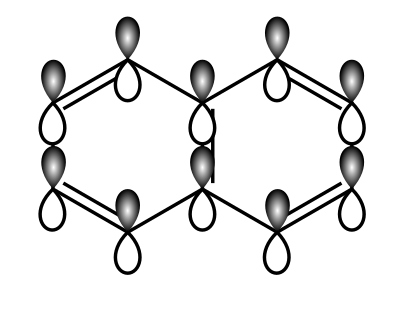
\includegraphics[scale=0.72]{./structures/exercise_1/naphthalene/10.png}
			\captionof*{figure}{$\varepsilon = \alpha + 2.303\beta$}
			\end{minipage} & 
			\begin{minipage}[t]{0.175\linewidth}
			\setlength{\abovecaptionskip}{0.5em}
			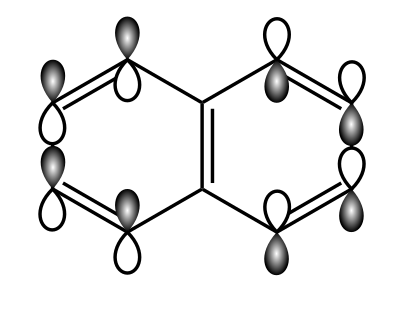
\includegraphics[scale=0.72]{./structures/exercise_1/naphthalene/2.png}
			\captionof*{figure}{$\varepsilon = \alpha + 1.618\beta$}
			\end{minipage} &
			\begin{minipage}[t]{0.175\linewidth}
			\centering
			\setlength{\abovecaptionskip}{0.5em}\hspace*{-0.6em}
			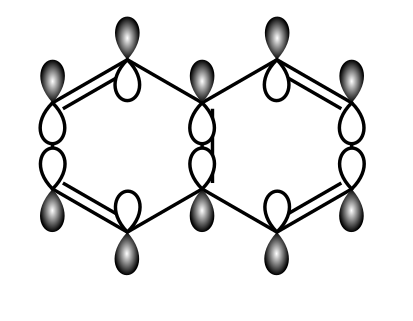
\includegraphics[scale=0.72]{./structures/exercise_1/naphthalene/5.png}
			\captionof*{figure}{$\varepsilon = \alpha + 1.303\beta$}
			\end{minipage} & 
			\begin{minipage}[t]{0.175\linewidth}
			\setlength{\abovecaptionskip}{0.5em}
			\vspace*{-4.8em}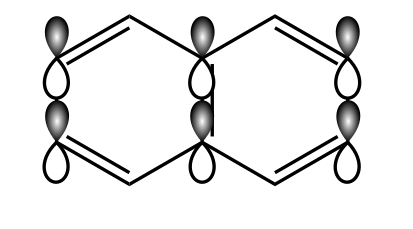
\includegraphics[scale=0.72]{./structures/exercise_1/naphthalene/8.png}\vspace*{0.85em}
			\captionof*{figure}{$\varepsilon = \alpha + 1.000\beta$}
			\end{minipage}
			\begin{minipage}[t]{0.175\linewidth}
			\setlength{\abovecaptionskip}{0.5em}
			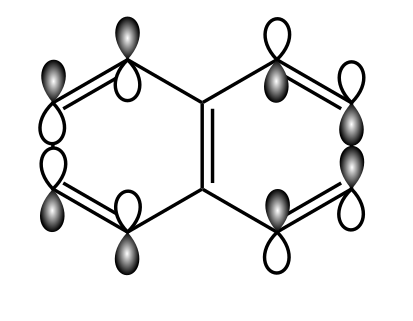
\includegraphics[scale=0.72]{./structures/exercise_1/naphthalene/7.png}\hspace*{-1.5em}
			\captionof*{figure}{$\varepsilon = \alpha + 0.618\beta$}
			\end{minipage} \\
			\begin{minipage}[t]{0.175\linewidth}
			\centering
			\setlength{\abovecaptionskip}{0.5em}
			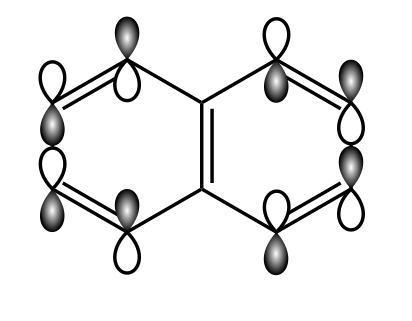
\includegraphics[scale=0.72]{./structures/exercise_1/naphthalene/1.png}
			\captionof*{figure}{$\varepsilon = \alpha -0.618 \beta$}
			\end{minipage} & 
			\begin{minipage}[t]{0.175\linewidth}
			\setlength{\abovecaptionskip}{0.5em}
			\vspace*{-4.7em}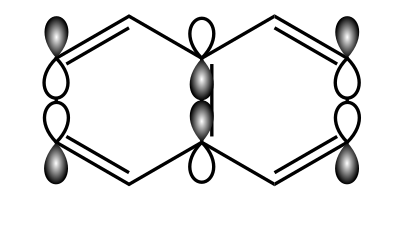
\includegraphics[scale=0.72]{./structures/exercise_1/naphthalene/3.png}\vspace*{0.7em}
			\captionof*{figure}{$\varepsilon = \alpha - 1.000\beta$}
			\end{minipage} &
			\begin{minipage}[t]{0.175\linewidth}
			\centering
			\setlength{\abovecaptionskip}{0.5em}
			\vspace*{-5.5em}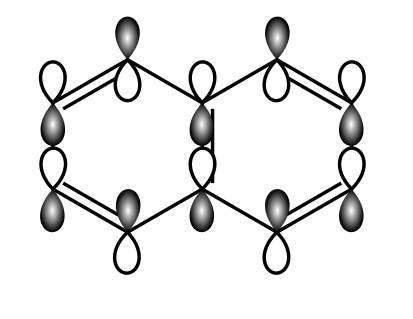
\includegraphics[scale=0.72]{./structures/exercise_1/naphthalene/9.png}
			\captionof*{figure}{$\varepsilon = \alpha - 1.303\beta$}
			\end{minipage} & 
			\begin{minipage}[t]{0.175\linewidth}
			\setlength{\abovecaptionskip}{0.5em}
			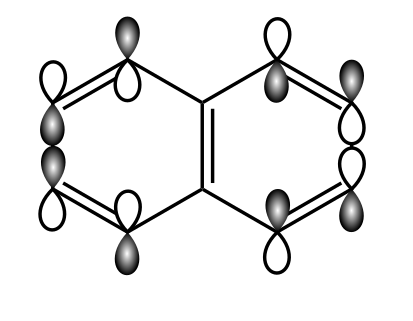
\includegraphics[scale=0.72]{./structures/exercise_1/naphthalene/6.png}\hspace*{-0.5em}
			\captionof*{figure}{$\varepsilon = \alpha - 1.618\beta$}
			\end{minipage}
			\begin{minipage}[t]{0.175\linewidth}
			\setlength{\abovecaptionskip}{0.5em}
			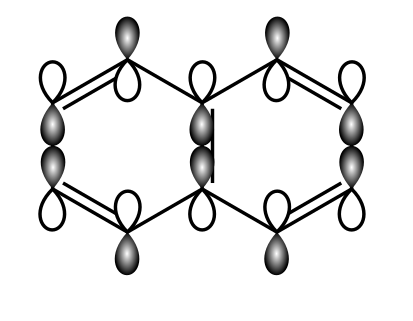
\includegraphics[scale=0.72]{./structures/exercise_1/naphthalene/4.png}\hspace*{-1.5em}
			\captionof*{figure}{$\varepsilon = \alpha - 2.303\beta$}
			\end{minipage}
		\end{tabular}				
		\captionof{figure}{Phase diagrams of these H{\"u}ckel MOs of naphthalene. Black bubbles mean plus phase while white ones mean minus phase. The color is used just for determining relative phase.}\label{fig:phase_diagram_5}
		\end{center}
		
		In the end, we conclude that for naphthalene, its ground state $\pi$-electron configuration is $(1b_{1u})^2 (1b_{2g})^2 (1b_{3g})^2 (2b_{1u})^2 (1a_u)^2$ and its delocalization energy is $2 \times 2.303 \beta + 2 \times 1.618 \beta + 2 \times 1.313 \beta + 2 \times 1.000 \beta + 2 \times 0.618 \beta - 10 \times 1.000 \beta = 3.684 \beta$, much larger than the sum of that of {\it trans}-1,3-butadiene ($0.472\beta$) and benzene ($2.000\beta$). 
		
		\begin{center}
		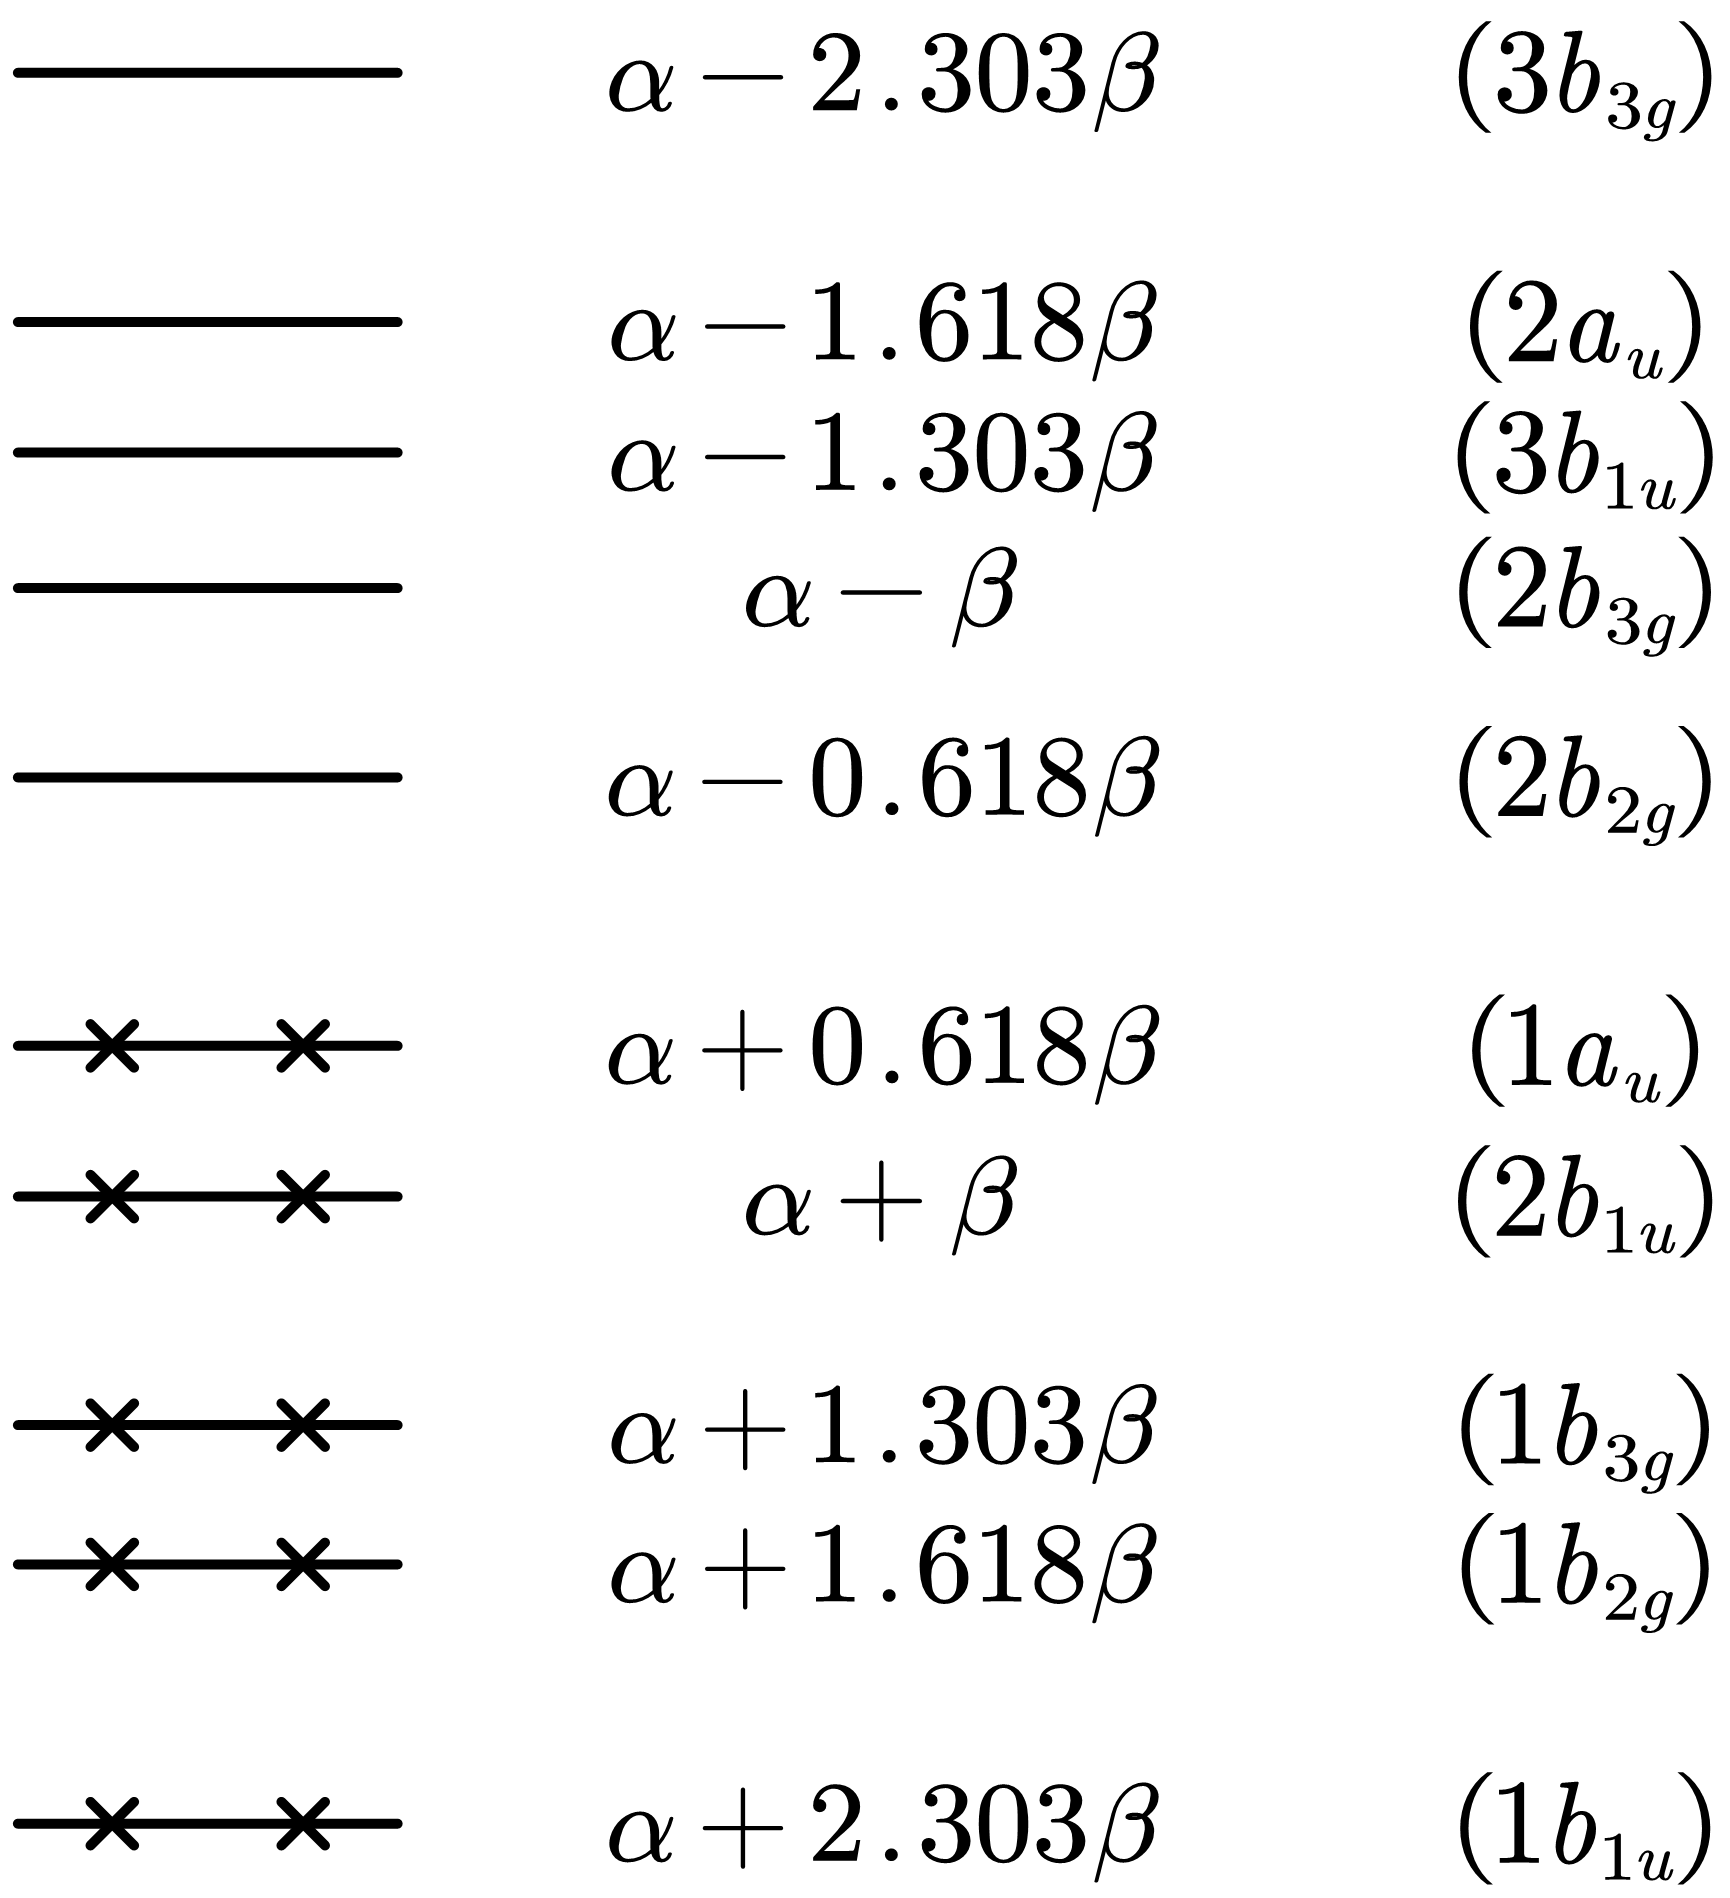
\includegraphics[scale=1.0]{./structures/exercise_1/naphthalene/998.png}
		\end{center}
		
		\item 66666666666666666	phenanthrene
		
		\begin{center}
		\begin{tabular}{ccccc}\hline
	$\mathscr{D}_{\rm 5}$ & $E$ & $C_2$ &	$\sigma_{xz}$	& $\sigma_{yz}$\\ \hline
			$A_1$	&	1	&	1	&	1	&	1	\\
			$A_2$	&	1	&	1	&	-1	&	-1	\\
			$B_1$ 	&	1	&	-1	&	1	&	-1	\\
			$B_2$ 	&	1	&	-1	&	-1	&	1	\\ \hline
		\end{tabular}
		\end{center}
		
		
		\begin{center}
		\begin{tabular}{ccccc}\hline
	$\mathscr{C}_{\rm 2v}$	& $E$ & $C_2$ &	$\sigma_{xz}$	& $\sigma_{yz}$ \\ \hline
	$\chi^{\AO}(C_i)$	&	14	&	0	&	0	&	-14	\\ \hline
		\end{tabular}
		\end{center}
			
		\begin{equation*}
		a_1 = 0, \quad a_2 = 7, \quad b_1 = 7, \quad b_2 = 0.
		\end{equation*}
		
		\begin{equation*}
			\Gamma^{\AO} = 7\Gamma^{A_2} \oplus 7\Gamma^{B_1}.
		\end{equation*}
		
		\begin{center}
		\begin{tabular}{ccccc}\hline
	$\mathscr{C}_{\rm 2v}$ & $E$ & $C_2$ &	$\sigma_{xz}$	& $\sigma_{yz}$	\\ \hline
			$\phi_1$	&	$\phi_1$	&	$-\phi_{10}$	&	$\phi_{10}$	&	$-\phi_1$	\\
			$\phi_2$	&	$\phi_2$	&	$-\phi_9$	&	$\phi_9$	&	$-\phi_2$		\\
			$\phi_3$	&	$\phi_3$	&	$-\phi_8$	&	$\phi_8$	&	$-\phi_3$		\\
			$\phi_4$	&	$\phi_4$	&	$-\phi_7$	&	$\phi_7$	&	$-\phi_4$		\\ 
			$\phi_5$	&	$\phi_5$	&	$-\phi_6$	&	$\phi_6$	&	$-\phi_5$		\\ 
			$\phi_{11}$	&	$\phi_{11}$	&	$-\phi_{14}$	&	$\phi_{14}$	&	$-\phi_{11}$		\\
			$\phi_{12}$	&	$\phi_{12}$	&	$-\phi_{13}$	&	$\phi_{13}$	&	$-\phi_{12}$		\\ \hline
		\end{tabular}
		\end{center}
		
		\end{enumerate}		
		
		
		\begin{equation*}
			\Hp_{A_2} = \begin{pmatrix}
\alpha&\beta&	0	&	0	&		0	&	-\beta 	&	0	\\
\beta&\alpha&\beta	&	0	&		0	&	0	&	0	\\
0	&\beta	&\alpha	&\beta	&		0	&	0	&	0	\\
0	&	0	&\beta	&\alpha	&	\beta	&	0	&	0	\\
0	&	0	&	0	&\beta	&\alpha-\beta&	-\beta	&	0\\
-\beta&	0	&	0	&	0	& -\beta	&	\alpha	&	\beta \\
0	&	0	&	0	&	0	&	0		&	\beta	&\alpha-\beta\\
			\end{pmatrix}					
		\end{equation*}
		
		\begin{equation*}
			\Hp_{B_1} = \begin{pmatrix}
\alpha&\beta&	0	&	0	&		0	&	\beta 	&	0	\\
\beta&\alpha&\beta	&	0	&		0	&	0	&	0	\\
0	&\beta	&\alpha	&\beta	&		0	&	0	&	0	\\
0	&	0	&\beta	&\alpha	&	\beta	&	0	&	0	\\
0	&	0	&	0	&\beta	&\alpha+\beta&	\beta	&	0\\
\beta&	0	&	0	&	0	& \beta		&	\alpha	&	\beta \\
0	&	0	&	0	&	0	&	0		&	\beta	&\alpha+\beta\\
			\end{pmatrix}					
		\end{equation*}
		
	\end{solution}

\end{document}